\subsection{The order function}

Let A be a filtered ring, E a filtered A-module and \((\mathrm{E}_{n})\) the filtration of E. For all \(x \in E\) let \(v(x)\) denote the least upper bound in \(\bar{R}\) of the set on integers \(n \in Z\) such that \(x \in E_{n}\) . Then the following equivalences hold:

\[
\left\{ \begin{array}{l} v (x) = - \infty \Leftrightarrow x \notin \bigcup_ {n \in \mathbf {Z}} \mathrm{E} _ {n} \\ v (x) = p \quad \Leftrightarrow x \in \mathrm{E} _ {p} \quad \text { and } \quad x \notin \mathrm{E} _ {p + 1} \\ v (x) = + \infty \Leftrightarrow x \in \bigcap_ {n \in \mathbf {Z}} \mathrm{E} _ {n} \end{array} \right.\tag{4}
\]

The mapping \(v: \mathrm{E} \to \overline{\mathbf{R}}\) is called the order function of the filtered module \(\mathrm{E}\) . If \(v\) is known then so are the \(\mathrm{E}_n\) , for \(\mathrm{E}_n\) is the set of \(x \in \mathrm{E}\) such that \(v(x) \geqslant n\) ; the fact that the \(\mathrm{E}_n\) are additive subgroups of \(\mathrm{E}\) implies the relation

\[
v (x - y) \geqslant \inf (v (x), v (y)).\tag{5}
\]

The above definition applies in particular to the filtered A-module \(A_{s}\) ; let w be its order function. It follows from equation (3) of no. 1 that for \(a \in A\) and \(x \in E\) ,

\[
v (a x) \geqslant w (a) + v (x)\tag{6}
\]

whenever the right-hand side is defined; in particular, for \(a \in A\) and \(b \in A\) ,

\[
w (a b) \geqslant w (a) + w (b)\tag{7}
\]

whenever the right hand side is defined.

The order function is defined similarly on a filtered group G which is not necessarily commutative; the corresponding relation to (5) is then written

\[
v (y x ^ {- 1}) = v (x y ^ {- 1}) \geqslant \inf (v (x), v (y)).\tag{5'}
\]

\subsection{The graded module associated with a filtered module}

Let G be a commutative group (written additively) and \((G_{n})\) a filtration on G. Let us write

\[
\begin{array}{l} \operatorname{gr} _ {n} (\mathbf {G}) = \mathbf {G} _ {n} / \mathbf {G} _ {n + 1} \quad \text { for } \quad n \in \mathbf {Z} \\ \operatorname{gr} (\mathbf {G}) = \bigoplus_ {n \in \mathbf {Z}} \operatorname{gr} _ {n} (\mathbf {G}). \end{array}\tag{8}
\]

The commutative group \(\operatorname{gr}(\mathbf{G})\) is then a graded group of type \(\mathbf{Z}\) , called the graded group associated with the filtered group \(\mathbf{G}\) , the homogeneous elements of degree \(n\) of \(\operatorname{gr}(\mathbf{G})\) being those of \(\operatorname{gr}_n(\mathbf{G})\) .

Now let A be a filtered ring, \((\mathbf{A}_{n})\) its filtration, E a filtered A-module and \((\mathbf{E}_{n})\) its filtration. For all \(p \in Z\) , \(q \in Z\) , a mapping

\[
\operatorname{gr} _ {p} (\mathrm{A}) \times \operatorname{gr} _ {q} (\mathrm{E}) \rightarrow \operatorname{gr} _ {p + q} (\mathrm{E})\tag{9}
\]

is defined as follows: given \(\alpha \in \mathrm{gr}_p(\mathbf{A})\) , \(\xi \in \mathrm{gr}_q(\mathbf{E})\) , two representatives \(a, a'\) of \(\alpha\) and two representatives \(x, x'\) of \(\xi\) , \(ax \in \mathrm{E}_{p + q}\) , \(a'x' \in \mathrm{E}_{p + q}\) and \(ax \equiv a'x'\) (mod. \(\mathrm{E}_{p + q + 1}\) ), for

\[
a x - a ^ {\prime} x ^ {\prime} = (a - a ^ {\prime}) x + a ^ {\prime} (x - x ^ {\prime})
\]

and \(a - a' \in \mathbf{A}_{p+1}\) and \(x - x' \in \mathbf{E}_{q+1}\) and hence our assertion follows from formula (3) of no. 1. We may therefore denote by \(\alpha\xi\) the class in

\[
\mathbf {E} _ {p + 1} / \mathbf {E} _ {p + q + 1} = \operatorname{gr} _ {p + q} (\mathbf {E})
\]

of the product ax of any representative \(a \in \alpha\) and any representative \(x \in \xi\) . It is immediate that the mapping (9) is Z-bilinear; by linearity, we derive a Z-bilinear mapping

\[
\operatorname{gr} (\mathrm{A}) \times \operatorname{gr} (\mathrm{E}) \rightarrow \operatorname{gr} (\mathrm{E}).\tag{10}
\]

If this definition is first applied to the case \(E = A_{s}\) , the mapping (10) is an internal law of composition on \(\mathrm{gr}(A)\) , which it is immediately verified is associative and has an identity element which is the canonical image in \(\mathrm{gr}_{0}(A)\) of the unit element of A; it therefore defines on \(\mathrm{gr}(A)\) a ring structure and the graduation \((\mathrm{gr}_{n}(A))_{n\in\mathbf{Z}}\) is by definition compatible with this structure. The graded ring \(\mathrm{gr}(A)\) (of type Z) thus defined is called the graded ring associated with the filtered ring A; it is obviously commutative if A is commutative; \(\mathrm{gr}_{0}(A)\) is a subring of \(\mathrm{gr}(A)\) . The mapping (10) is on the other hand a \(\mathrm{gr}(A)\) -module external law on \(\mathrm{gr}(E)\) , the module axioms being trivially satisfied, and the graduation \((\mathrm{gr}_{n}(E))_{n\in\mathbf{Z}}\) on \(\mathrm{gr}(E)\) is obviously compatible with this module structure. The graded \(\mathrm{gr}(A)\) -module \(\mathrm{gr}(E)\) (of type Z) thus defined is called the graded module associated with the filtered A-module E.

\textbf{Examples}\par

\begin{enumerate}
\def\labelenumi{(\arabic{enumi})}
\item
  Let A be a commutative ring and t an element of A which is not a divisor of 0. Let us give A the \((t)\) -adic filtration (no. 1, Example 3). Then the associated graded ring \(\mathrm{gr}(\mathbf{A})\) is canonically isomorphic to the polynomial ring \((\mathbf{A}/(t))[\mathbf{X}]\) . For \(\mathrm{gr}_{n}(\mathbf{A}) = 0\) for n \textless{} 0 and by definition the ring \(\mathrm{gr}_{0}(\mathbf{A})\) is the ring \(\mathbf{A}/(t)\) . We now note that by virtue of the hypothesis on t the relation \(at^{n} \equiv 0 \pmod{t^{n+1}}\) is equivalent to \(a \equiv 0 \pmod{t}\) ; if \(\tau\) is the canonical image of t in \(\mathrm{gr}_{1}(\mathbf{A})\) , every element of \(\mathrm{gr}_{n}(\mathbf{A})\) may then be written uniquely in the form \(\alpha\tau^{n}\) where \(\alpha \in \mathrm{gr}_{0}(\mathbf{A})\) ; whence our assertion.
\item
  Let \(\mathbf{K}\) be a commutative ring, A the ring of formal power series

\[
\mathrm{K} \left[ \left[ \mathrm{X} _ {1}, \dots , \mathrm{X} _ {r} \right] \right]
\]

(Algebra, Chapter IV, § 5) and m the ideal of A whose elements are the formal power series with no constant term. Let us give A the m-adic filtration (no. 1, Example 3); if \(M_{1}, \ldots, M_{s}\) are the distinct monomials in \(X_{1}, \ldots, X_{r}\) of total degree n - 1, clearly every formal power series u of total order \(\omega(u) \geqslant n\)

(loc. cit., no. 2) may be written as \(\sum_{k=1} u_k M_k\) , where the \(u_k\) belong to \(m\) ; it is seen that \(m^n\) is the set of formal power series \(u\) such that \(\omega(u) \geqslant n\) , which shows that \(\omega\) is the order function for the m-adic filtration. Then clearly, for every formal power series \(u \in m^n\) , there exists a unique homogeneous polynomial of degree \(n\) in the \(X_i\) which is congruent to \(u\) mod. \(m^{n+1}\) , namely the sum of terms of degree \(n\) of \(u\) ; we conclude that \(\text{gr}(A)\) is canonically isomorphic to the polynomial ring \(K[X_1, \ldots, X_f]\) .

\item
  More generally, let A be a commutative ring, b an ideal of A and A be given the b-adic filtration. If we write \(\mathbf{B} = \mathbf{gr}_{0}(\mathbf{A})\) , \(\mathbf{F} = \mathbf{gr}_{1}(\mathbf{A}) = \mathbf{b}/\mathbf{b}^{2}\) , we know (Algebra, Chapter III,) that the identity mapping of the B-module F onto itself can be extended uniquely to a homomorphism u from the symmetric algebra \(\mathbf{S}(\mathbf{F})\) of F to the B-algebra \(\mathbf{gr}(\mathbf{A})\) ; it follows from the definition of \(\mathbf{gr}(\mathbf{A})\) that u is a surjective homomorphism of graded algebras; for \(n \geqslant 1\) , every element of \(\mathbf{gr}_{n}(\mathbf{A})\) is a sum of classes mod \(b^{n+1}\) of elements of the form \(y = x_{1}x_{2}\ldots x_{n}\) , where \(x_{i} \in b (1 \leqslant i \leqslant n)\) ; if \(\xi_{i}\) is the class of \(x_{i} \mod b^{2}\) , clearly the class of y mod. \(b^{n+1}\) is the element \(u(\xi_{1})\ldots u(\xi_{n})\) , whence our assertion. In particular, every system of generators of the B-module F is a system of generators of the B-algebra \(\mathbf{gr}(\mathbf{A})\) .
\end{enumerate}

If now E is an A-module and E is given the b-adic filtration, it is seen similarly that the graded gr(A)-module gr(E) is generated by gr₀(E) = E/bE. To be precise, the restriction φ to gr(A) × gr₀(E) of the external law on the gr(A)-module gr(E) is a Z-bilinear mapping of gr(A) × gr₀(E) to gr(E); moreover gr(A) is a (gr₀(A), gr₀(A))-bimodule and gr₀(E) a gr₀(A)-module; it is immediately verified that, for α ∈ gr(A), α₀ ∈ gr₀(A), ξ ∈ gr₀(E),

\[
\phi (\alpha \alpha_ {0}, \xi) = \phi (\alpha , \alpha_ {0} \xi)
\]

and hence \(\phi\) defines a surjective \(\mathbf{gr}_0(\mathbf{A})\) -linear mapping

\[
\gamma_ {\mathrm{E}} \colon \operatorname{gr} (\mathrm{A}) \otimes_ {\mathbf {g r} _ {0} (\mathrm{A})} \operatorname{gr} _ {0} (\mathrm{E}) \rightarrow \operatorname{gr} (\mathrm{E})\tag{11}
\]

which is called canonical.

* (4) Let K be a commutative ring, g a Lie algebra over K and U the enveloping algebra of g. An increasing filtration \((\mathrm{U}_{n})_{n\in\mathbf{Z}}\) is defined on U by taking \(U_{n}=\{0\}\) for n\textless0 and denoting by \(U_{n}\) for \(n\geqslant0\) the set of elements of U which can be expressed as a sum of products of at most n elements of g; then

\(U_{0} = K\) and \(\text{gr}(U)\) is a commutative K-algebra (Lie Groups and Lie Algebras, Chapter I, § 2, no. 6). The canonical mapping of \(g\) to \(\text{gr}_{1}(U) = U_{1}/U_{0}\) can be extended uniquely to a homomorphism \(h\) of the symmetric algebra \(S(g)\) of the K-module \(g\) to the K-algebra \(\text{gr}(U)\) ; the homomorphism \(h\) is surjective and, if the K-module \(g\) is free, \(h\) is bijective (loc. cit., no. 7, Theorem 1).

\begin{enumerate}
\def\labelenumi{(\arabic{enumi})}
\setcounter{enumi}{4}
\tightlist
\item
  Let A be a graded ring of type Z and E a graded A-module of type Z; let \(A_{(i)}\) (resp. \(E_{(i)}\) ) be the subgroup of homogeneous elements of degree i of A (resp. E). Let A and E be given the filtrations associated with their graduations (no. 1, Example 1) and let \(A'\) and \(E'\) denote the filtered ring and filtered \(A'\) -module thus obtained. Then it is immediate that the Z-linear mapping \(A \to \text{gr}(A')\) which maps an element of \(A_{(n)}\) to its canonical image in

\[
\operatorname{gr} _ {n} (\mathbf {A}) = \left(\bigoplus_ {i \geqslant n} \mathbf {A} _ {(i)}\right) / \left(\bigoplus_ {i \geqslant n + 1} \mathbf {A} _ {(i)}\right)
\]

is a graded ring isomorphism. A canonical graded A-module isomorphism \(\mathbf{E} \to \mathrm{gr}(\mathbf{E}')\) is defined similarly.
\end{enumerate}

PROPOSITION 1. Let A be a filtered ring, \((\mathbf{A}_n)_{n\in \mathbf{Z}}\) its filtration and \(v\) its order function. Suppose that \(\operatorname {gr}(\mathbf{A})\) is a ring with no divisor of zero. Then, for every ordered pair of elements \(a,b\) of the ring \(\mathbf{B} = \bigcup_{n\in \mathbf{Z}}\mathbf{A}_n,v(ab) = v(a) + v(b)\) .

As \(n = \bigcap_{n \in \mathbf{Z}} A_n\) is a two-sided ideal of the ring \(B\) , the formula holds if \(v(a)\) or \(v(b)\) is equal to \(+\infty\) . If not, \(v(a) = r\) and \(v(b) = s\) are integers; the classes \(\alpha\) of \(a \bmod A_{r+1}\) and \(\beta\) of \(b \bmod A_{s+1}\) are \(\neq 0\) by definition, whence by hypothesis \(\alpha \beta \neq 0\) in \(\operatorname{gr}(A)\) and therefore \(ab \notin A_{r+s+1}\) ; as \(ab \in A_{r+s}\) ,

\[
v (a b) = v (a) + v (b).
\]

COROLLARY. Let A be a filtered ring and \((\mathbf{A}_{n})_{n\in\mathbf{Z}}\) its filtration; let us set \(B=\bigcup_{n\in Z}A_{n}\) , \(n=\bigcap_{n\in Z}A_{n}\) . If the ring gr(A) has no divisors of zero, neither has the ring B/n.

If \(a\) and \(b\) are elements of \(B\) not belonging to \(\mathfrak{n}\) , then \(v(a) \neq +\infty\) and \(v(b) \neq +\infty\) , whence \(v(ab) \neq +\infty\) and therefore \(ab \notin \mathfrak{n}\) .

Note that the ring A can be an integral domain and the filtration \((A_{n})\) exhaustive and separated without gr(A) being an integral domain (Exercise 2).

Remark. Let G be a group which is not necessarily commutative with a filtration \((\mathrm{G}_{n})_{n\in\mathbf{Z}}\) such that \(G_{n+1}\) is normal in \(G_{n}\) for all \(n\in Z\) ; again let \(\mathrm{gr}_{n}(\mathrm{G})=\mathrm{G}_{n}/\mathrm{G}_{n+1}\) . The restricted product of the family \((\mathrm{gr}_{n}(\mathrm{G}))_{n\in\mathbf{Z}}\) , that is the subgroup of the product \(\prod_{n\in\mathbf{Z}}\mathrm{gr}_{n}(\mathrm{G})\) consisting of the elements \((\xi_{n})\) all of whose components, except at most a finite number, are equal to the identity element, is also called the graded group associated with G and denoted by \(\mathrm{gr}(\mathrm{G})\) .

\subsection{Homomorphisms compatible with filtrations}

Let \(G, G'\) be two commutative groups (written additively), \((G_n)\) a filtration on \(G\) and \((G'_n)\) a filtration on \(G'\) ; a homomorphism \(h: G \to G'\) is called compatible with the filtrations on \(G\) and \(G'\) if \(h(G_n) \subset G'_n\) for all \(n \in \mathbf{Z}\) . The composite homomorphism \(G_n \xrightarrow{h|G_n} G'_n \longrightarrow G'_n / G_{n+1}'\) is zero on \(G_{n+1}\) and hence defines by taking quotients a homomorphism \(h_n: G_n / G_{n+1} \to G'_n / G_{n+1}'\) ; there is therefore a unique additive group homomorphism \(\text{gr}(h): \text{gr}(G) \to \text{gr}(G')\) such that, for all \(n \in \mathbf{Z}\) , \(\text{gr}(h)\) coincides with \(h_n\) on \(\text{gr}_n(G) = G_n / G_{n+1}\) . \(\text{gr}(h)\) is called the graded group homomorphism associated with \(h\) . If \(G''\) is a third filtered group and \(h': G' \to G''\) a homomorphism which is compatible with the filtrations, \(h' \circ h\) is a homomorphism which is compatible with the filtrations and

\[
\operatorname{gr} (h ^ {\prime} \circ h) = \operatorname{gr} (h ^ {\prime}) \circ \operatorname{gr} (h).\tag{12}
\]

PROPOSITION 2. Let G be a filtered commutative group and H a subgroup of G; let H be given the induced filtration and G/H the quotient filtration. If j: H → G is the canonical injection and p: G → G/H the canonical surjection, j and p are compatible with the filtrations and the sequence

\[
0 \longrightarrow \operatorname{gr} (\mathrm{H}) \xrightarrow {\operatorname{gr} (j)} \operatorname{gr} (\mathrm{G}) \xrightarrow {\operatorname{gr} (p)} \operatorname{gr} (\mathrm{G} / \mathrm{H}) \longrightarrow 0\tag{13}
\]

is exact.

The first assertion is obvious; if \((\mathbf{G}_n)\) is the filtration on \(\mathbf{G}\) , then

\[
\left(\mathrm{H} \cap \mathrm{G} _ {n}\right) \cap \mathrm{G} _ {n + 1} = \mathrm{H} \cap \mathrm{G} _ {n + 1}
\]

and hence \(\mathrm{gr}(j)\) is injective; moreover the canonical mapping

\[
\mathrm{G} _ {n} \rightarrow (\mathrm{H} + \mathrm{G} _ {n}) / \mathrm{H}
\]

is surjective, hence so is \(\operatorname{gr}(p)\) and \(\operatorname{gr}(p) \circ \operatorname{gr}(j) = 0\) by (12). Finally, let \(\xi \in \mathbf{G}_n / \mathbf{G}_{n+1}\) belong to the kernel of \(\operatorname{gr}(p)\) ; then there exists \(x \in \xi\) such that \(x \in \mathbf{H} + \mathbf{G}_{n+1}\) ; but as \(\mathbf{G}_{n+1} \subset \mathbf{G}_n\) ,

\[
\mathrm{G} _ {n} \cap (\mathrm{H} + \mathrm{G} _ {n + 1}) = (\mathrm{H} \cap \mathrm{G} _ {n}) + \mathrm{G} _ {n + 1}
\]

and hence \(x = y + z\) where \(y \in \mathbf{H} \cap \mathbf{G}_n\) and \(z \in \mathbf{G}_{n+1}\) ; this proves that \(\xi\) is the class mod. \(\mathbf{G}_{n+1}\) of \(j(y)\) , in other words it belongs to the image of \(\operatorname{gr}(\mathbf{H})\) under \(\operatorname{gr}(j)\) .

Note that, given an exact sequence \(0 \to G' \xrightarrow{u} G \xrightarrow{v} G'' \to 0\) of filtered commutative groups, where \(u\) and \(v\) are compatible with the filtrations, the sequence \(0 \longrightarrow \text{gr}(G') \xrightarrow{\text{gr}(u)} \text{gr}(G) \xrightarrow{\text{gr}(v)} \text{gr}(G'') \longrightarrow 0\) is not necessarily exact (Exercise 4).

If now A and B are two filtered rings and \(h \colon \mathbf{A} \to \mathbf{B}\) a ring homomorphism which is compatible with the filtrations, it is immediately verified that the graded group homomorphism \(\mathrm{gr}(h) \colon \mathrm{gr}(\mathbf{A}) \to \mathrm{gr}(\mathbf{B})\) is also a ring homomorphism. In particular, if \(\mathbf{A}'\) is a subring of A with the induced filtration, \(\mathrm{gr}(\mathbf{A}')\) is canonically identified with a graded subring of \(\mathrm{gr}(\mathbf{A})\) (Proposition 2); if \(\mathfrak{b}\) is a two-sided ideal of A and \(\mathbf{A} / \mathfrak{b}\) is given the quotient filtration, \(\mathrm{gr}(\mathbf{A} / \mathfrak{b})\) is canonically identified with the quotient graded ring \(\mathrm{gr}(\mathbf{A}) / \mathrm{gr}(\mathfrak{b})\) (Proposition 2).

Finally, let A be a filtered ring, E, F two filtered A-modules and \(u: \mathbf{E} \to \mathbf{F}\) an homomorphism compatible with the filtrations. Then it is immediate that \(\mathrm{gr}(u): \mathrm{gr}(\mathrm{E}) \to \mathrm{gr}(\mathrm{F})\) is a \(\mathrm{gr}(\mathrm{A})\) -linear mapping and hence a homogeneous homomorphism of degree 0 of graded \(\mathrm{gr}(\mathrm{A})\) -modules. Moreover, if \(u': \mathbf{E} \to \mathbf{F}\) is another A-homomorphism compatible with the filtrations, so is \(u + u'\) and

\[
\operatorname{gr} (u + u ^ {\prime}) = \operatorname{gr} (u) + \operatorname{gr} (u ^ {\prime}).\tag{14}
\]

\textbf{Remarks}\par

\begin{enumerate}
\def\labelenumi{(\arabic{enumi})}
\item
  Clearly filtered ring homomorphisms (resp. homomorphisms of filtered modules over a given filtered ring A) compatible with the filtrations can be taken as morphisms for the filtered ring structure (resp. filtered A-module structure) (Set Theory, Chapter IV, § 2, no. 1).
\item
  Let E and F be two modules over a filtered ring A and let them have the filtrations derived from the filtration \((\mathbf{A}_{n})\) on A (no. 1, Example 2). Then every A-linear mapping \(u: E \rightarrow F\) is compatible with the filtrations, since

\[
u (\mathrm{A} _ {n} \mathrm{E}) = \mathrm{A} _ {n} u (\mathrm{E}) \subset \mathrm{A} _ {n} \mathrm{F}.
\]

\item
  Note that a filtered A-module homomorphism \(u: \mathbf{E} \to \mathbf{F}\) which is compatible with the filtrations may satisfy \(\operatorname{gr}(u) = 0\) without being zero; this is so for example of the endomorphism \(x \mapsto nx\) of the additive group \(\mathbf{Z}\) with the \((n)\) -adic filtration (for any integer \(n > 1\) ). The relation \(\operatorname{gr}(u) = \operatorname{gr}(v)\) for two homomorphisms \(u, v\) of \(\mathbf{E}\) to \(\mathbf{F}\) , compatible with the filtrations, does not therefore imply necessarily \(u = v\) .
\item
  The definitions at the beginning of this no. extend immediately to two groups G, G', which are not necessarily commutative and are filtered by subgroups Gn, Gn' such that Gn+1 (resp. Gn'+1) is normal in Gn (resp. Gn'). Proposition 2 is also valid with the same hypotheses on the Gn and assuming that H is invariant in G, the proof remaining unchanged except for notation.
\end{enumerate}

\subsection{The topology defined by a filtration}

Let \(\mathbf{G}\) be a group filtered by a family \((\mathbf{G}_n)_{n\in \mathbf{Z}}\) of normal subgroups of \(\mathbf{G}\) . There exists a unique topology on \(\mathbf{G}\) which is compatible with the group structure and for which the \(G_{n}\) constitute a fundamental system of neighbourhoods of the identity element e of G (General Topology, Chapter III, § 1, no. 2, Example); it is called the topology on G defined by the filtration ( \(G_{n}\) ). When we use topological notions concerning a filtered group, we shall mean, unless otherwise stated, with the topology defined by the filtration. Note that the \(G_{n}\) , being subgroups of G, are both open and closed (General Topology, Chapter III, § 2, no. 1, Corollary to Proposition 4).

As each \(G_{n}\) is normal in G, the entourages of the left and right uniformities on G coincide; we deduce that G admits a Hausdorff completion group \(\hat{G}\) (General Topology, Chapter III, § 3, no. 4, Theorem 1 and no. 1, Proposition 2).

For every subset M of G, the closure of M in G is equal to

\[
\bigcap_ {n \in \mathbf {Z}} (\mathbf {M}. \mathbf {G} _ {n}) = \bigcap_ {n \in \mathbf {Z}} (\mathbf {G} _ {n}. \mathbf {M})
\]

(General Topology, Chapter III, § 3, no. 1, formula (1)); in particular \(\bigcap_{n\in\mathbf{Z}}\mathrm{G}_{n}\) is the closure of \(\{e\}\) ; thus it is seen that for the topology on \(\mathbf{G}\) to be Hausdorff it is necessary and sufficient that the filtration \((\mathrm{G}_{n})\) be separated. For the topology on \(\mathbf{G}\) to be discrete, it is necessary and sufficient that there exist \(n\in\mathbf{Z}\) such that \(\mathrm{G}_{n}=\{e\}\) (in which case \(\mathrm{G}_{m}=\{e\}\) for \(m\geqslant n\) ); then the filtration \((\mathrm{G}_{n})\) is called discrete.

Since the Hausdorff group associated with G is \(H = \frac{G}{\left(\bigcap_{n \in \mathbf{Z}} G_n\right)}\) , the associated graded groups \(\text{gr}(G)\) and \(\text{gr}(H)\) (if H is given the quotient filtration) are canonically identified.

Not let \(G'\) be another filtered group and \(u: G \to G'\) a homomorphism compatible with the filtrations; the definition of the topologies on G and \(G'\) shows immediately that u is continuous (*). If H is a subgroup (resp. normal subgroup) of G, the topology induced on H by that on G (resp. the quotient topology with respect to H of that on G) is the topology on H (resp. G/H) defined by the filtration induced by that on G (resp. quotient topology of that on G). The product topology of those on G and \(G'\) is the topology defined by the product of filtrations on G and \(G'\) .

Let \(v\) be the order function (no. 2) on \(G\) . The hypothesis on the \(G_n\) implies that \(v(xyx^{-1}) = v(y)\) and hence \(v(xy^{-1}) = v(yx^{-1}) = v(x^{-1}y) = v(y^{-1}x)\) for all \(x, y\) in \(G\) . Let \(\rho\) be a real number such that \(0 < \rho < 1\) (for example take \(\rho = 1 / e)\) and let \(d(x,y) = \rho^{y(xy - 1)}\) for all \(x,y\) in G. Then \(d(x,x) = 0, d(x,y) = d(y,x)\) and inequality (5') of no. 2 gives

\[
d (x, y) \leqslant \sup (d (x, z), d (y, z))\tag{15}
\]

for all x, y, z in G, which implies the triangle inequality

\[
d (x, y) \leqslant d (x, z) + d (y, z).
\]

Thus \(d\) is a pseudometric on G which is invariant under left and right translations and \(\mathbf{G}_n\) is the set of \(x \in \mathbf{G}\) such that \(d(e, x) \leqslant \rho^n\) ; the uniform structure defined by \(d\) is then the uniform structure on the topological group G. If G is Hausdorff, G is a zero-dimensional metrizable topological space (General Topology, Chapter IX, § 6, no. 4); \(d\) is a distance on G if also the filtration \((\mathbf{G}_n)\) is exhaustive.

Given a topological ring A, recall that a left topological A-module is an A-module E with a topology compatible with its additive group structure and such that the mapping \((a, x) \mapsto ax\) from A × E to E is continuous (General Topology, Chapter III, § 6, no. 6).

PROPOSITION 3. Let A be a filtered ring, \((\mathbf{A}_n)\) its filtration, B the subring \(\bigcup_{n\in \mathbf{Z}}\mathbf{A}_n\) of A, E a filtered B-module, \((\mathrm{E}_n)\) its filtration and F the sub-B-module \(\bigcup_{n\in \mathbf{Z}}\mathrm{E}_n\) of E. Then the mapping \((a,x)\mapsto ax\) from \(\mathbf{B}\times \mathbf{F}\) to F is continuous.

Let \(a_0 \in \mathbf{B}\) , \(x_0 \in \mathbf{F}\) ; there exists by hypothesis integers \(r, s\) such that \(a_0 \in \mathbf{A}_r\) and \(x_0 \in \mathbf{E}_s\) . The relation

\[
a x - a _ {0} x _ {0} = (a - a _ {0}) x _ {0} + a _ {0} (x - x _ {0}) + (a - a _ {0}) (x - x _ {0})
\]

shows that if \(a - a_0 \in \mathbf{A}_l\) and \(x - x_0 \in \mathrm{E}_f\) , \(ax - a_0x_0\) belongs to

\[
\mathbf {E} _ {i + s} + \mathbf {E} _ {j + r} + \mathbf {E} _ {i + j}.
\]

Then, given an integer \(n\) , \(ax - a_0x_0 \in \mathrm{E}_n\) provided \(i \geqslant n - s\) , \(j \geqslant n - r\) and \(i + j \geqslant n\) , that is so long as \(i\) and \(j\) are sufficiently large.

COROLLARY. The ring B is a topological ring and the B-module F a topological B-module.

The first assertion is obtained by applying Proposition 3 to \(\mathbf{F} = \mathbf{B}_s\) .

It is seen in particular that a filtered ring A whose filtration is exhaustive is a topological ring; if this is so every filtered A-module whose filtration is exhaustive is a topological A-module.

PROPOSITION 4. Let A be a commutative ring filtered by an exhaustive filtration \((\mathbf{A}_n)\) and \(\mathfrak{p}\) an ideal of A. Suppose that the ideal \(\operatorname{gr}(\mathfrak{p}) = \bigoplus_{n \in \mathbf{Z}} (\mathfrak{p} \cap \mathbf{A}_n) / (\mathfrak{p} \cap \mathbf{A}_{n+1})\) of the ring \(\operatorname{gr}(\mathbf{A})\) is prime. Then the closure of \(\mathfrak{p}\) in A is a prime ideal.

We know that \(\operatorname{gr}(\mathbf{A} / \mathfrak{p})\) is isomorphic to \(\operatorname{gr}(\mathbf{A}) / \operatorname{gr}(\mathfrak{p})\) (no. 4, Proposition 2) and hence an integral domain; we conclude that \(\mathbf{A} / \bigcap_{n\in \mathbf{Z}}(\mathfrak{p} + \mathbf{A}_n)\) is an integral domain (no. 3, Corollary to Proposition 1). Then the closure \(\bigcap_{n\in \mathbf{Z}}(\mathfrak{p} + \mathbf{A}_n)\) of \(\mathfrak{p}\) is a prime ideal.

Let A be a ring and m a two-sided ideal of A; the topology defined on A by the m-adic filtration (no. 1, Example 3) is called the m-adic topology; as the m-adic filtration is exhaustive, A is a topological ring with this topology (Corollary to Proposition 3). Similarly, for every A-module E, the topology defined by the m-adic filtration is called the m-adic topology on E; E is a topological A-module under this topology.

Let \(m'\) be another two-sided ideal of A; for the \(m'\) -adic topology on A to be finer than the \(m\) -adic topology, it is necessary and sufficient that there exist an integer n \textgreater{} 0 such that \(m'^n \subset m\) ; the condition is necessary and, if it is fulfilled, \(m'^{hn} \subset m^h\) for all h \textgreater{} 0 and hence the condition is sufficient. If A is a commutative Noetherian ring, it amounts to the same to say that \(V(m) \subset V(m')\) in the prime spectrum of A (Chapter II, § 4, no. 3, Corollary 2 to Proposition 11 and § 2, no. 6, Proposition 15).

\subsection{Complete filtered modules}

PROPOSITION 5. Let G be a filtered group whose filtration (G \(_{n}\) ) consists of invariant subgroups of G. The following conditions are equivalent:

\begin{enumerate}
\def\labelenumi{(\alph{enumi})}
\item
  G is a complete topological group.
\item
  The associated Hausdorff group \(\mathbf{G}' = \mathbf{G} / \left(\bigcap_{n\in \mathbf{Z}}\mathbf{G}_n\right)\) is complete.
\item
  Every Cauchy sequence in G is convergent.
\end{enumerate}

If \(\mathbf{G}\) is commutative and written additively, these conditions are also equivalent to the following:

\begin{enumerate}
\def\labelenumi{(\alph{enumi})}
\setcounter{enumi}{3}
\tightlist
\item
  Every family \((x_{\lambda})_{\lambda \in L}\) of elements of \(\mathbf{G}'\) which converges to 0 with respect to the filter \(\mathfrak{F}\) of complements of finite subsets of \(\mathbf{L}\) is summable in \(\mathbf{G}'\) .
\end{enumerate}

For a filter on G to be a Cauchy filter (resp. a convergent filter), it is necessary and sufficient that its image under the canonical mapping \(G \rightarrow G'\) be a Cauchy (resp. convergent) filter (General Topology, Chapter II, §3, no. 1, Proposition 4); whence first of all the equivalence of (a) and (b); on the other hand, as \(G'\) is metrizable, the equivalence of (b) and (c) follows from Proposition 9 of General Topology, Chapter IX, §2, no. 6.

Suppose now that \(G\) is commutative. Suppose that \(G'\) is complete and let \((x_{\lambda})_{\lambda \in L}\) be a family of elements of \(G'\) which converge to 0 with respect to \(\mathfrak{F}\) . For every neighbourhood \(V'\) of 0 in \(G'\) which is a subgroup of \(G'\) , there exists a finite subset \(J\) of \(L\) such that the condition \(\lambda \in L - J\) implies \(x_{\lambda} \in V'\) ; then \(\sum_{\lambda \in H} x_{\lambda} \in V'\) for every finite subset \(H\) of \(L\) not meeting \(J\) , which shows that the family \((x_{\lambda})_{\lambda \in L}\) is summable (General Topology, Chapter III, § 5, no. 2, Theorem 1).

Conversely, suppose that condition (d) holds and let \((x_{n})\) be a Cauchy sequence on \(G'\) ; the family \((x_{n+1} - x_{n})\) is then summable and in particular the series with general term \(x_{n+1} - x_{n}\) is convergent and hence the sequence \((x_{n})\) is convergent.

Let G be a filtered group whose filtration \((\mathbf{G}_{n})\) consists of normal subgroups of G; the quotient groups \(G/G_{n}\) are discrete and hence complete, since the \(G_{n}\) are open in G. Let \(f_{n}\) be the canonical mapping \(G \to G/G_{n}\) and for \(m \leqslant n\) let \(f_{mn}\) be the canonical mapping \(G/G_{n} \to G/G_{m}\) ; \((\mathbf{G}/\mathbf{G}_{n}, f_{mn})\) is an inverse system of discrete groups with Z as indexing set (General Topology, Chapter III, §7, no. 3). Let \(\tilde{G}\) be the topological group the inverse limit of this inverse system and for all n let \(g_{n}: \tilde{G} \to G/G_{n}\) be the canonical mapping; let \(f: G \to \tilde{G}\) be the inverse limit of the inverse system of mappings \((f_{n})\) such that \(f_{n} = g_{n} \circ f\) for all n; finally, let j be the canonical mapping of G to its Hausdorff completion \(\hat{G}\) ; as the \(G/G_{n}\) are complete, there exists a unique topological group isomorphism i: \(\hat{G} \to \tilde{G}\) such that \(f = i \circ j\) (loc. cit., Corollary 1 to Proposition 2); we shall call it the canonical isomorphism of \(\hat{G}\) onto \(\tilde{G}\) .

Let H be another filtered group whose filtration \((\mathbf{H}_{n})\) consists of normal subgroups of H and let \(u: G \to H\) be a homomorphism compatible with the filtrations (no. 4). Set \(\tilde{H} = \lim H/H_{n}\) ; for all n, u defines by taking quotients a homomorphism \(u_{n}: G/G_{n} \xleftarrow{\leftarrow} H/H_{n}\) and the \(u_{n}\) obviously form an inverse system of mappings; set \(\tilde{u} = \lim u_{n}\) . Moreover let \(\tilde{H}\) be the Hausdorff completion of H and \(\hat{u}: \hat{G} \to \hat{H}\) the homomorphism derived from u by passing to the Hausdorff completions (General Topology, Chapter II, § 3, no. 7, Proposition 15). It follows immediately from the definitions that if \(\tilde{G}\) is identified with \(\tilde{G}\) and \(\tilde{H}\) with \(\tilde{H}\) by means of the canonical isomorphisms, \(\hat{u}\) is identified with \(\tilde{u}\) . We conclude in particular that, if, for all n, \(u_{n}\) is an isomorphism, then \(\hat{u}\) is an isomorphism of topological groups.

\textbf{Examples of complete filtered groups and rings}\par

\begin{enumerate}
\def\labelenumi{(\arabic{enumi})}
\item
  Let G be a complete filtered group. Every closed subgroup of G with the induced filtration is complete (General Topology, Chapter II, § 3, no. 4, Proposition 8). Every quotient group of G with the quotient filtration is complete (General Topology, Chapter IX, § 3, no. 1, Remark 1).
\item
  Let A be a filtered commutative ring whose filtration we denote by \((a_n)_{n\in \mathbf{Z}}\) ; let \(A'\) be the ring of formal power series \(A[[X_1,\ldots ,X_s]]\) . For all \(e = (e_1,\dots ,e_s)\in \mathbf{N}^s\) , we write \(|e| = \sum_{i\in 1}^{s}e_i\) , \(X^e = \prod_{i\in 1}^{s}X_i^{e_i}\) so that every element \(P\in A'\) can be written uniquely \(P = \sum_{e\in \mathbf{N}^s}\alpha_{e,P}X^e\) where \(\alpha_{e,P}\in A\) . For all \(n\in \mathbf{Z}\) , let \(\mathfrak{a}_n'\) denote the set of \(\mathrm{P} \in \mathrm{A}'\) such that \(\alpha_{e,\mathrm{P}} \in \mathfrak{a}_{n-|e|}\) for all \(e \in \mathbf{N}^s\) ; we show that \(\mathfrak{a}_n'\) is an ideal of \(\mathrm{A}'\) . Clearly \(\mathfrak{a}_n'\) is an additive subgroup of \(\mathrm{A}'\) ; on the other hand, if \(\mathrm{P} \in \mathfrak{a}_n'\) and \(\mathrm{Q} \in \mathrm{A}'\) , then, for all \(e \in \mathbf{N}^s\) , \(\alpha_{e,\mathrm{PQ}} = \sum_{e' + e'' = e} \alpha_{e',\mathrm{Q}} \alpha_{e'',\mathrm{P}}\) ; as the relation \(e' + e'' = e\) implies \(|e''| \leqslant |e|\) , \(\mathrm{PQ} \in \mathfrak{a}_n'\) . Moreover, if \(\mathrm{Q} \in \mathfrak{a}_m'\) , then, for \(e' + e'' = e\) , \(\alpha_{e',\mathrm{Q}} \alpha_{e'',\mathrm{P}} \in \mathfrak{a}_{m-|e'|} \mathfrak{a}_{n-|e''}| \subset \mathfrak{a}_{m+n-|e|}\) , which proves that \((\mathfrak{a}_n')_{n \in \mathbf{Z}}\) is a filtration compatible with the ring structure on \(\mathrm{A}'\) (for obviously \(1 \in \mathfrak{a}_0'\) ). When in future we speak of \(\mathrm{A}'\) as a filtered ring, we shall mean, unless otherwise stated, with the filtration \((\mathfrak{a}_n')\) . Clearly \(\bigcap_{n \in \mathbf{Z}} \mathfrak{a}_n'\) is the set of formal power series all of whose coefficients belong to \(\bigcap_{n \in \mathbf{Z}} \mathfrak{a}_n\) ; then, if A is Hausdorff, so is \(\mathrm{A}'\) . If \(\mathfrak{a}_0 = \mathrm{A}\) , then \(\mathfrak{a}_0' = \mathrm{A}'\) .
\end{enumerate}

PROPOSITION 6. With the above notation, suppose that \(\mathfrak{a}_0 = \mathbf{A}\) and let \(h\) denote the mapping \(\mathbf{P} \mapsto (\alpha_{e,\mathbf{P}})_{e \in \mathbb{N}^s}\) . Then \(h\) is an isomorphism of the additive topological group \(\mathbf{A}'\) onto the additive topological group \(\mathbf{A}^{\mathbf{N}^s}\) . The polynomial ring \(\mathbf{A}[\mathbf{X}_1, \ldots, \mathbf{X}_s]\) is dense in \(\mathbf{A}'\) ; if \(\mathbf{A}\) is complete, so is \(\mathbf{A}'\) .

Clearly \(h\) is bijective; \(V_n = h(a_n')\) is the set of \((a_e) \in A^{N^s}\) such that \(a_e \in a_{n-|e|}\) for all \(e \in N^s\) such that \(|e| \leqslant n\) ; as these elements \(e\) are finite in number, \(V_n\) is a neighbourhood of 0 in \(A^{N^s}\) . Conversely, if \(V\) is a neighbourhood of 0 in \(A^{N^s}\) , there is a finite subset \(E\) of \(N^s\) and an integer \(v\) such that the conditions \(a_e \in a_v\) for all \(e \in E\) imply \((a_e) \in V\) ; if then \(n\) is the greatest of the integers \(v + |e|\) for \(e \in E\) , then \(h(a_n') \subset V\) , which proves the first assertion of Proposition 6. Moreover, with \(n\) and \(E\) defined as above, \(h(P - \sum_{e \in E} \alpha_{e, P} X^e) \in V\) for all \(P \in A'\) , which shows that \(A[X_1, \ldots, X_s]\) is dense in \(A'\) . The last assertion follows from the first and the fact that a product of complete spaces is complete.

Let \(m\) be an ideal of \(A\) and suppose that \((\mathfrak{a}_n)\) is the \(m\) -adic filtration; then, if \(n\) is the ideal of \(A'\) generated by \(m\) and the \(X_i\) ( \(1 \leqslant i \leqslant s\) ), the filtration \((\mathfrak{a}_n')\) is the \(n\) -adic filtration. For clearly, for all \(k \geqslant 0\) , \(n^k\) is generated by the elements \(aX^e\) such that \(a \in m^{k-|e|}\) for all \(e \in N^s\) such that \(|e| \leqslant k\) , whence \(n^k \subset \mathfrak{a}_k'\) . Let us prove conversely that \(\mathfrak{a}_k' \subset n^k\) . For all \(P \in \mathfrak{a}_k'\) , \(P = P' + P''\) , where \(P' = \sum_{|e| < k} \alpha_{e,P} X^e\) , \(P'' = \sum_{|e| \geqslant k} \alpha_{e,P} X^e\) . Clearly it is possible to write \(P'' = \sum_{|e|=k} X^e Q_e\) , where the \(Q_e\) are elements of \(A'\) , whence \(P'' \in n^k\) ; on the other hand, clearly \(\alpha_{e,P} X^e \in n^k\) for all \(e \in N^s\) , whence \(P' \in n^k\) . Then \(n^k = \mathfrak{a}_k'\) .

COROLLARY. Let A be a commutative ring,

\[
\mathbf {A} ^ {\prime} = \mathbf {A} [ [ \mathbf {X} _ {1}, \dots , \mathbf {X} _ {s} ] ]
\]

the ring of formal power series in s indeterminates over A and n the ideal of \(\Lambda'\) consisting of the formal power series with no constant term. The ring \(\Lambda'\) is Hausdorff and complete with the n-adic topology and the polynomial ring \(\mathbf{A}[\mathbf{X}_1,\dots ,\mathbf{X}_s]\) is everywhere dense in \(\mathbf{A}'\) .

It is sufficient to apply what has just been said to the case \(\mathfrak{m} = \{0\}\) .

\subsection{Linear compactness properties of complete filtered modules}

Recall that, if E is an A-module, an affine subset (or an affine linear variety) of E is any subset F which is empty or of the form \(a + M\) , where \(a \in E\) and M is a submodule of E called the direction of F (Algebra, Chapter II, § 9, nos. 1 and 3).

PROPOSITION 7. Let A be a filtered ring, E a filtered A-module and \((\mathbf{E}_{n})\) the filtration of E; suppose that \(E_{0} = E\) , that the \(E_{n}\) are submodules of E, that the A-modules \(E/E_{n}\) are Artinian and finally that the topological group E is Hausdorff and complete. Then the intersection of a decreasing sequence of non-empty closed affine subsets of E is non-empty.

We have seen in no. 6 that, since E is Hausdorff and complete, it is identified with \(\tilde{\mathbf{E}} = \varprojlim \mathrm{E} / \mathrm{E}_n\) . Let \((\mathbf{W}_p)\) be a decreasing sequence of non-empty closed affine subsets of E and, for all \(n \geqslant 0\) , let \(\mathbf{W}_{p,n}\) be the canonical image of \(\mathbf{W}_p\) in \(\mathrm{E} / \mathrm{E}_n\) ; we are going to construct a sequence \(x = (x_n) \in \tilde{\mathbf{E}}\) such that \(x_n \in \mathbf{W}_{p,n}\) for all \(p\) and all \(n\) ; hence \(x \in \mathbf{W}_p + \mathbf{E}_n\) for all \(p\) and all \(n\) and, as the \(\mathbf{W}_p\) are closed, \(x \in \mathbf{W}_p\) for all \(p\) (no. 5), which will prove the proposition.

As \(E/E_{0}=0\) , we shall take \(x_{0}=0\) . Suppose that the \(x_{i}\) are defined for \(0\leqslant i\leqslant n-1\) and let \(W_{p,n}^{\prime}\) be the set of elements of \(W_{p,n}\) whose canonical image in \(E/E_{n-1}\) is \(x_{n-1}\) ; as \(x_{n-1}\in W_{p,n-1}\) and \(W_{p,n-1}\) is the canonical image of \(W_{p,n}\) , \(W_{p,n}^{\prime}\) is non-empty and is obviously an affine subset of \(E/E_{n}\) ; moreover the sequence \((W_{p,n}^{\prime})_{p\in\mathbf{N}}\) is decreasing. As \(E/E_{n}\) is Artinian, this sequence is stationary (otherwise the sequence of submodules of \(E/E_{n}\) which are the directions of the \(W_{p,n}^{\prime}\) would be strictly decreasing, which is absurd). It is sufficient then to take \(x_{n}\) to be an element of \(\bigcap_{p\in\mathbf{N}}W_{p,n}^{\prime}\) and the construction of \((x_{n})\) can then be performed by induction.

PROPOSITION 8. Suppose that A and E satisfy the hypotheses of Proposition 7. Let \((\mathbf{F}_{p})\) be a decreasing sequence of closed submodules of E such that \(\bigcap_{p} F_{p} = 0\) . Then, for every neighbourhood V of 0 in E, there exists p such that \(F_{p} \subset V\) (in other words, the base of the filter \((\mathbf{F}_{p})\) converges to 0).

We may assume that V is one of the \(E_{n}\) , in which case E/V is Artinian. Let us write \(F_{p}^{\prime} = (F_{p} + V)/V\) ; as the \(F_{p}^{\prime}\) form a decreasing sequence of submodules of E/V, there exists an integer j such that \(F_{p}^{\prime} = F_{j}^{\prime}\) for all \(p \geqslant j\) . We shall see that \(F_{j}^{\prime} = \{0\}\) , which will complete the proof. Let \(x \in F_{j}^{\prime}\) and let \(W_{p}\) be the set of elements of \(F_{p}\) whose image in E/V is \(x (p \geqslant j)\) ; by definition of j, the \(W_{p}\) are non-empty closed affine subsets of E and obviously \(W_{p+1} \subset W_{p}\) ;

then it follows from Proposition 7 that there exists an element \(y\) belonging to all the \(W_p\) . As \(W_p \subset F_p\) and \(\bigcap_{p \in \mathbf{N}} F_p = \{0\}\) , \(y = 0\) ; since \(x\) is the canonical image of \(y\) in \(E / V\) , \(x = 0\) (cf.~Exercises 15 to 21).

\subsection{The lift of homomorphisms of associated graded modules}

THEOREM 1. Let X, Y be two filtered groups whose filtrations \((\mathbf{X}_n)\) , \((\mathbf{Y}_n)\) consist of normal subgroups; let \(u: \mathbf{X} \to \mathbf{Y}\) be a homomorphism compatible with the filtrations.

\begin{enumerate}
\def\labelenumi{(\roman{enumi})}
\item
  Suppose that the filtration \((\mathbf{X}_n)\) is exhaustive. For \(\operatorname{gr}(u)\) to be injective, it is necessary and sufficient that \(u^{-1}(\mathbf{Y}_n) = \mathbf{X}_n\) for all \(n \in \mathbf{Z}\) .
\item
  Suppose that one of the following hypotheses holds: (α) X is complete and Y Hausdorff; (β) Y is discrete. Then, for gr(u) to be surjective, it is necessary and sufficient that \(Y_{n} = u(X_{n})\) for all \(n \in Z\) .
\end{enumerate}

\begin{enumerate}
\def\labelenumi{(\roman{enumi})}
\tightlist
\item
  To say that the mapping \(\mathbf{gr}_n(u)\) is injective means that

\[
\mathbf {X} _ {n} \cap^ {- 1} u ^ {1} (\mathbf {Y} _ {n + 1}) \subset \mathbf {X} _ {n + 1}.
\]

This is obviously the case of \(\bar{u}^1 (\mathbf{Y}_{n + 1}) = \mathbf{X}_{n + 1}\) . Conversely, if

\[
\mathbf {X} _ {n} \cap^ {- 1} u (\mathbf {Y} _ {n + 1}) \subset \mathbf {X} _ {n + 1}
\]

for all \(n\) , we deduce by induction on \(k\) that \(\mathbf{X}_{n-k} \cap \bar{u}^1(\mathbf{Y}_{n+1}) \subset \mathbf{X}_{n+1}\) for all \(n \in \mathbf{Z}\) and all \(k \geqslant 0\) . As the filtration \((\mathbf{X}_n)\) is exhaustive, we see that, for all \(n\) , \(\mathbf{X}\) is the union of the \(\mathbf{X}_{n-k} (k \geqslant 0)\) , hence \(\bar{u}^1(\mathbf{Y}_{n+1}) \subset \mathbf{X}_{n+1}\) for all \(n\) and therefore \(\mathbf{X}_{n+1} \subset \bar{u}^1(\mathbf{Y}_{n+1})\) , which completes the proof.

\item
  To say that the mapping \(\mathrm{gr}_n(u)\) is surjective means that
\end{enumerate}

\[
\mathbf {Y} _ {n} = u (\mathbf {X} _ {n}) \mathbf {Y} _ {n + 1}.
\]

This is obviously the case if \(Y_{n}=u(X_{n})\) . Conversely, suppose that \(Y_{n}=u(X_{n})Y_{n+1}\) for all \(n\in Z\) . Let n be an integer and y an element of \(Y_{n}\) ; we shall define a sequence \((x_{k})_{k\geq0}\) of elements of \(X_{n}\) such that \(x_{k}\in X_{n}\) , \(x_{k+1}\equiv x_{k} \pmod{X_{n+k}}\) and \(u(x_{k})\equiv y \pmod{Y_{n+k}}\) for all \(k\geq0\) . We shall take \(x_{0}\) equal to the identity element of X, which certainly gives \(u(x_{0})\equiv y \pmod{Y_{n}}\) . Suppose that an \(x_{k}\in X_{n}\) has been constructed such that \(u(x_{k})\equiv y \pmod{Y_{n+k}}\) ; then \((u(x_{k}))^{-1}y\in Y_{n+k}\) ; the hypothesis implies that there exists \(t\in X_{n+k}\) such that \(u(t)\equiv(u(x_{k}))^{-1}y \pmod{Y_{n+k+1}}\) and hence \(u(x_{k}t)\equiv y \pmod{Y_{n+k+1}}\) ; it is sufficient to take \(x_{k+1}=x_{k}t\) to carry out the induction. This being so, if Y is discrete, there exists \(k\geq0\) such that \(Y_{n+k}=\{e'\}\) (the identity element of Y), whence \(u(x_{k})=y\) and hence in this case it has been proved that \(u(X_{n})=Y_{n}\) for all n.~Suppose now that X is complete and Y Hausdorff. As \(x_{h}^{-1}x_{k}\in X_{n+k}\) for \(h\geq k\geq0\) , \((x_{k})\) is a Cauchy sequence in \(X_{n}\) ; as

\(X_{n}\) is closed in X and hence complete, this sequence has at least one limit x in \(X_{n}\) . By virtue of the continuity of u, \(u(x)\) is the unique limit of the sequence \((u(x_{k}))\) in Y, Y being Hausdorff. But the relations \(u(x_{k}) \equiv y \pmod{Y_{n+k+1}}\) show that y is also a limit of this sequence, whence \(u(x) = y\) and it has also been proved that \(u(X_{n}) = Y_{n}\) .

COROLLARY 1. Suppose that X is Hausdorff and its filtration exhaustive. Then, if gr(u) is injective, u is injective.

Let \(e, e'\) be the identity elements of X and Y respectively. Then

\[
\bar {u} ^ {1} (e ^ {\prime}) \subset \bigcap_ {n} \bar {u} ^ {1} (\mathbf {Y} _ {n}) = \bigcap_ {n} \mathbf {X} _ {n} = \{e \}
\]

by hypothesis, whence the corollary.

COROLLARY 2. Suppose that one of the following hypotheses holds:

(α) X is complete, Y is Hausdorff and its filtration is exhaustive;

(β) Y is discrete and its filtration is exhaustive.

Then, if \(\operatorname{gr}(u)\) is surjective, \(u\) is surjective.

In this case \(\mathbf{Y} = \bigcup_{n}\mathbf{Y}_{n} = \bigcup_{n}u(\mathbf{X}_{n})\subset u(\mathbf{X}).\)

COROLLARY 3. Suppose that X and Y are Hausdorff, the filtrations of X and Y exhaustive and X complete. Then, if gr(u) is bijective, u is bijective.

Let A be a local ring, m its maximal ideal and M an A-module; let A and M be given the m-adic filtrations and let gr(A) and gr(M) be the graded ring and the graded gr(A)-module associated with A and M. We have seen (no. 3, Example 3) that the canonical mapping (11) is always surjective; we are going to consider the following property of M:

(GR) The canonical mapping

\[
\gamma_ {\mathbf {M}} \colon \operatorname{gr} (\mathbf {A}) \otimes_ {\mathbf {g r} _ {0} (\mathbf {A})} \operatorname{gr} _ {0} (\mathbf {M}) \rightarrow \operatorname{gr} (\mathbf {M})
\]

is bijective.

PROPOSITION 9. Let A be a local ring, m its maximal ideal, M, N two A-modules and u: N → M an A-homomorphism. M and N are given the m-adic filtrations and suppose that: (1) M satisfies property (GR); (2) gr₀(u): gr₀(N) → gr₀(M) is injective. Then gr(u): gr(N) → gr(M) is injective, N and P = Coker(u) satisfy property (GR) and mⁿN = -¹u(mⁿM) for every integer n \textgreater{} 0.

It is immediately verified that the diagram

\[
\begin{array}{c} \operatorname{gr} (\mathrm{A}) \otimes_ {\mathbf {g r} _ {0} (\mathrm{A})} \operatorname{gr} _ {0} (\mathrm{N}) \xrightarrow {1 \otimes \operatorname{gr} _ {0} (u)} \operatorname{gr} (\mathrm{A}) \otimes_ {\mathbf {g r} _ {0} (\mathrm{A})} \operatorname{gr} _ {0} (\mathrm{M}) \\ \gamma_ {\mathrm{N}} \Biggl \downarrow \\ \operatorname{gr} (\mathrm{N}) \xrightarrow [ \operatorname{gr} (u) ]{} \operatorname{gr} (\mathrm{M}) \end{array}
\]

is commutative. As \(\mathrm{gr}_{0}(\mathbf{A}) = \mathbf{A}/\mathfrak{m}\) is a field, the hypothesis implies that \(1 \otimes \mathrm{gr}_{0}(u)\) is injective; as by hypothesis \(\gamma_{M}\) is injective, so is \(\gamma_{M} \circ (1 \otimes \mathrm{gr}_{0}(u))\) . This implies first that \(\gamma_{N}\) is injective and hence bijective and therefore that \(\mathrm{gr}(u)\) is injective. The formula \(\overline{u}^{1}(\mathfrak{m}^{n}\mathbf{M}) = \mathfrak{m}^{n}\mathbf{N}\) is then a consequence of Theorem 1 (i).

Also, let us write \(N' = u(N)\) and let \(j: N' \to M\) be the canonical injection. If \(p: M \to P = M/N'\) is the canonical homomorphism, then in the commutative diagram

\pandocbounded{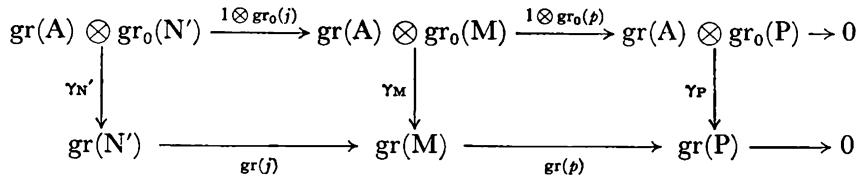
\includegraphics[keepaspectratio]{images/part002_c4775371.jpg}}

the lower row is exact (no. 4, Proposition 2) and so is the upper row by virtue of Proposition 2 of no. 4 and the fact that \(\mathrm{gr}_0(\mathbf{A})\) is a field. Moreover, \(\mathrm{gr}(j)\) is injective (no. 4, Proposition 2) and hence \(\mathrm{gr}_0(j)\) is injective. The first part of the argument applied to \(j\) shows that \(\gamma_{\mathbf{N}'}\) is bijective; as \(\gamma_{\mathbf{M}}\) is also bijective by hypothesis, we conclude that \(\gamma_{\mathbf{P}}\) is bijective (Chapter I, § 1, no. 4, Corollary 2 to Proposition 2).

COROLLARY. Under the hypotheses of Proposition 9, if we assume also that N is Hausdorff with the m-adic filtration, then u is injective.

This follows from the fact that \(\operatorname{gr}(u)\) is injective (Corollary 1 to Theorem 1).

* Remark. Suppose that the hypotheses of Proposition 9 hold and also one of the following conditions:

\begin{enumerate}
\def\labelenumi{(\arabic{enumi})}
\item
  m is nilpotent;
\item
  A is Noetherian and P is ideally Hausdorff (cf.~§ 5, no. 1);
\end{enumerate}

then P is a flat A-module. This follows from the fact that \(\gamma_{P}\) is bijective and § 5, no. 2, Theorem 1 (iv), since A/m is a field. *

\subsection{The lift of families of elements of an associated graded module}

Let A be a filtered commutative ring, \((\mathbf{A}_{n})_{n\in\mathbf{Z}}\) its filtration and C a subring of \(A_{0}\) such that \(C\cap A_{1}=\{0\}\) . The restriction to C of the canonical mapping \(\mathbf{A}_{0}\to\mathbf{A}_{0}/\mathbf{A}_{1}=\mathrm{gr}_{0}(\mathbf{A})\) is then injective, which allows us to identify C with a submodule of \(\mathrm{gr}_{0}(\mathbf{A})\) ; this is what we shall usually do in similar cases. If \(A_{1}\neq A_{0}\) and K is any subfield of \(A_{0}\) , then \(K\cap A_{1}=\{0\}\) since \(K\cap A_{1}\) is an ideal of K not containing 1; then K may be identified with a subfield of \(\mathrm{gr}_{0}(\mathbf{A})\) .

PROPOSITION 10. Let A be a filtered commutative ring and \((\mathbf{A}_n)\) its filtration; suppose that there exists a subring \(\mathbf{C}\) of \(\mathbf{A}_0\) such that \(\mathbf{C} \cap \mathbf{A}_1 = \{0\}\) and \(\mathbf{C}\) is identified with a subring of \(\operatorname{gr}_0(\mathbf{A})\) . Let \((x_i)_{1 \leqslant i \leqslant q}\) be a finite family of elements of \(\mathbf{A}\) ; suppose that \(x_i \in \mathbf{A}_{n_i}\) for \(1 \leqslant i \leqslant q\) and let \(\xi_i\) be the class of \(x_i\) in \(\operatorname{gr}_{n_i}(\mathbf{A})\) for \(1 \leqslant i \leqslant q\) .

\begin{enumerate}
\def\labelenumi{(\roman{enumi})}
\item
  If the family \((\xi_{i})\) of elements of \(\operatorname{gr}(\mathbf{A})\) is algebraically free over \(\mathbf{C}\) , the family \((x_{i})\) is algebraically free over \(\mathbf{C}\) .
\item
  If the filtration on \(\mathbf{A}\) is exhaustive and discrete and \((\xi_{i})\) is a system of generators of the C-algebra \(\operatorname{gr}(\mathbf{A})\) , then \((x_{i})\) is a system of generators of the C-algebra \(\mathbf{A}\) .
\end{enumerate}

Let \(\mathbf{A}'\) be the polynomial algebra \(\mathbf{C}[\mathbf{X}_1, \ldots, \mathbf{X}_q]\) over \(\mathbf{C}\) ; let \(\mathbf{A}'\) be given the graduation \((\mathbf{A}_n')\) of type \(\mathbf{Z}\) where \(\mathbf{A}_n'\) is the set of C-linear combinations of the monomials \(\mathbf{X}_1^{s(1)} \ldots \mathbf{X}_q^{s(q)}\) such that \(\sum_{i=1}^{q} n_i s(i) = n\) . Let \(u\) be the homomorphism \(f \mapsto f(x_1, \ldots, x_q)\) from the C-algebra \(\mathbf{A}'\) to the C-algebra \(\mathbf{A}\) ; by definition, \(u(\mathbf{A}_n') \subset \mathbf{A}_n\) for all \(n \in \mathbf{Z}\) and hence \(u\) is compatible with the filtrations ( \(\mathbf{A}'\) being given its filtered ring structure associated with its graded ring structure, cf.~no. 1, Example 1). This being so, the hypothesis of (i) means that

\[
\operatorname{gr} (u): \mathrm{A} ^ {\prime} = \operatorname{gr} (\mathrm{A} ^ {\prime}) \rightarrow \operatorname{gr} (\mathrm{A})
\]

is injective; as the filtration on A' is exhaustive and separated, Corollary 1 to Theorem 1 of no. 8 may be applied and u is injective, which proves the conclusion of (i). Similarly, the hypothesis (ii) on the \((\xi_{i})\) means that gr(u) is surjective; as A is discrete and its filtration is exhaustive, Corollary 2 to Theorem 1 of no. 8 may be applied and u is surjective, which proves the conclusion of (ii).

PROPOSITION 11. Let A be a complete Hausdorff filtered commutative ring, C a subring of \(\mathbf{A}_0\) such that \(\mathbf{C} \cap \mathbf{A}_1 = 0\) and \((x_i)_{1 \leqslant i \leqslant q}\) a finite family of elements of A such that \(x_i \in \mathbf{A}_{n_i}\) where \(n_i > 0\) for \(1 \leqslant i \leqslant q\) ; let \(\xi_i\) be the class of \(x_i\) in \(\operatorname{gr}_{n_i}(\mathbf{A})\) for \(1 \leqslant i \leqslant q\) . (i) There exists a unique C-homomorphism \(v\) from the algebra of formal power series \(\mathbf{A}'' = \mathbf{C}[[\mathbf{X}_1, \ldots, \mathbf{X}_q]]\) to A such that \(v(\mathbf{X}_i) = x_i\) for \(1 \leqslant i \leqslant q\) .

\begin{enumerate}
\def\labelenumi{(\roman{enumi})}
\setcounter{enumi}{1}
\item
  If the family \((\xi_{i})\) is algebraically free over \(\mathbf{C}\) , the homomorphism \(v\) is injective.
\item
  If the filtration on \(\mathbf{A}\) is exhaustive and the family \((\xi_{i})\) is a system of generators of the C-algebra \(\operatorname{gr}(\mathbf{A})\) , the homomorphism \(v\) is surjective.
\end{enumerate}

As \(n_i \geqslant 1\) for all \(i, \sum_{i=1}^{q} n_i s(i) \geqslant \sum_{i=1}^{q} s(i)\) for every monomial \(X_1^{s(1)} \ldots X_q^{s(q)}\) and on the other hand \(\sum_{i=1}^{q} n_i s(i) \leqslant r. \sum_{i=1}^{q} s(i)\) if \(r\) is the greatest of the \(n_i\) . If \(A_n''\) denotes the set of formal power series whose non-zero terms \(a_s X_1^{s(1)} \ldots X_q^{s(q)}\) satisfy \(\sum_{i=1}^{q} n_i s(i) \geqslant n\) , it follows from no. 6, Corollary to Proposition 6 that \(A''\) is Hausdorff and complete with the exhaustive filtration \((A_n'')\) and that

\[
\mathrm{A} ^ {\prime} = \mathrm{C} [ \mathrm{X} _ {1}, \dots , \mathrm{X} _ {q} ]
\]

is dense in A''; moreover the homomorphism u defined in the proof of Proposition 10 is continuous on A' and can be extended uniquely to a continuous homomorphism v: A''→A, since A is Hausdorff and complete (General Topology, Chapter III, § 3, no. 3, Proposition 5), which proves (i); also, gr(A'') = gr(A') and gr(v) = gr(u); (ii) and (iii) then follow respectively from Corollaries 1 and 2 to Theorem 1 of no. 8 in view of the hypotheses on A.

The conclusion of (ii) (resp. (iii)) of the proposition is sometimes expressed by saying that the family \((x_{i})\) is formally free over C (resp. a formal system of generators of A).

PROPOSITION 12. Let A be a filtered ring, E a filtered A-module and \((\mathbf{A}_{n})\) and \((\mathbf{E}_{n})\) the respective filtrations on A and E. Suppose that A is complete and the filtration \((\mathbf{E}_{n})\) is exhaustive and separated. Let \((x_{i})_{i\in\mathbf{I}}\) be a finite family of elements of E and for \(i\in I\) let \(n(i)\) be an integer such that \(x_{i}\in\mathbf{E}_{n(i)}\) ; finally let \(\xi_{i}\) be the class of \(x_{i}\) in \(\mathrm{gr}_{n(i)}(\mathbf{E})\) . Then, if \((\xi_{i})\) is a system of generators of the gr(A)-module gr(E), \((x_{i})\) is a system of generators of the A-module E.

In the A-module \(\mathbf{L} = \mathbf{A}_s^{\mathbf{I}}\) let \(\mathbf{L}_n\) denote the set \((a_i)\) such that \(a_i \in \mathbf{A}_{n - n(i)}\) for all \(i \in \mathbf{I}\) ; if \(p\) and \(q\) are the least and greatest of the \(n(i)\) , then \(\mathbf{A}_{n - q}^{\mathbf{I}} \supset \mathbf{L}_n \supset \mathbf{A}_{n - p}^{\mathbf{I}}\) and the topology defined on \(\mathbf{L}\) by the definition \((\mathbf{L}_n)\) is the same as the product topology; hence \(\mathbf{L}\) is a complete filtered A-module. As \(\mathbf{L}\) is free, there exists an

A-linear mapping \(u: \mathbf{L} \to \mathbf{E}\) such that \(u((a_i)) = \sum_{i \in \mathbf{I}} a_i x_i\) and it is obviously compatible with the filtrations; we must prove that \(u\) is surjective and for this it is sufficient, by virtue of Corollary 2 to Theorem 1, no. 8, to show that

\[
\operatorname{gr} (u): \operatorname{gr} (\mathbf {L}) \rightarrow \operatorname{gr} (\mathbf {E})
\]

is surjective or also that, for all \(x \in \mathbf{E}_n\) , there exist a family \((a_i)\) such that \(a_i \in \mathbf{A}_{n-n(i)}\) for all \(i \in I\) and \(x \equiv \sum_{i \in I} a_i x_i \pmod{\mathbf{E}_{n+1}}\) . Let \(\xi\) be the class of \(x\) in \(\mathrm{gr}_n(\mathbf{E})\) ; since the \(\xi_i\) generate the \(\mathrm{gr}(\mathbf{A})\) -module \(\mathrm{gr}(\mathbf{E})\) , there exist \(\alpha_i \in \mathrm{gr}(\mathbf{A})\) such that \(\xi = \sum_{i \in I} \alpha_i \xi_i\) and we may assume that \(\alpha_i \in \mathrm{gr}_{n-n(i)}(\mathbf{A})\) by replacing if need be \(\alpha_i\) by its homogeneous component of degree \(n - n(i)\) . Then \(\alpha_i\) is the image of an element \(a_i \in \mathbf{A}_{n-n(i)}\) and the family \((a_i)\) has the required property.

COROLLARY 1. Let A be a complete filtered ring and E a filtered A-module whose filtration is exhaustive and separated. If gr(E) is a finitely generated (resp. Noetherian) gr(A)-module, then E is a finitely generated (resp. Noetherian) A-module.

If \(\mathrm{gr}(\mathrm{E})\) is finitely generated, there is a finite system of homogeneous generators and Proposition 12 shows that E is finitely generated. Suppose now that \(\mathrm{gr}(\mathrm{E})\) is Noetherian and let F be a submodule of E; the filtration induced on F by that on E is exhaustive and separated and \(\mathrm{gr}(\mathrm{F})\) is identified with a sub-gr(A)-module of gr(E) (no. 4, Proposition 2) and hence is finitely generated by hypothesis; we conclude that F is a finitely generated A-module and hence E is Noetherian.

COROLLARY 2. Let A be a complete Hausdorff filtered ring whose filtration is exhaustive. If gr(A) is a left Noetherian ring, so is A.

It is sufficient to apply Corollary 1 with \(\mathbf{E} = \mathbf{A}_s\) .

COROLLARY 3. Let A be a complete filtered ring, \((\mathbf{A}_{n})\) its filtration, E a Hausdorff filtered A-module, \((\mathbf{E}_{n})\) its filtration and F a finitely generated submodule of E; suppose that \(A_{0} = A\) and \(E_{0} = E\) .

\begin{enumerate}
\def\labelenumi{(\roman{enumi})}
\item
  If, for all \(k \geqslant 0\) , \(\mathbf{E}_k = \mathbf{E}_{k+1} + \mathbf{A}_k\mathbf{F}\) , then \(\mathbf{F} = \mathbf{E}\) .
\item
  If it is further supposed that the filtration on \(\mathbf{E}\) is derived from that on \(\mathbf{A}\) (no. 1, Example 2), the relation \(\mathbf{E} = \mathbf{E}_1 + \mathbf{F}\) implies \(\mathbf{F} = \mathbf{E}\) .
\end{enumerate}

Let \(\xi_{i}(1\leqslant i\leqslant n)\) be the classes mod. \(\mathbf{E}_1\) of a finite system of generators of \(\mathbf{F}\) . It follows from the given hypothesis that for all \(k\geqslant 0\) every element of \(\mathrm{gr}_k(\mathrm{E})\)

can be expressed in the form \(\sum_{i=1}^{\infty} \alpha_i \xi_i\) where \(\alpha_i \in \mathrm{gr}(A)\) ; the \(\xi_i\) therefore generate the \(\mathrm{gr}(A)\) -module \(\mathrm{gr}(E)\) , which proves (i) by virtue of Proposition 12. If the filtration on \(E\) is derived from that on \(A\) , the relation \(E = E_1 + F\) implies

\[
\begin{array}{r} \mathbf {E} _ {k} = \mathbf {A} _ {k} \mathbf {E} = \mathbf {A} _ {k} \mathbf {E} _ {1} + \mathbf {A} _ {k} \mathbf {F} = \mathbf {A} _ {k} \mathbf {A} _ {1} \mathbf {E} + \mathbf {A} _ {k} \mathbf {F} \subset \mathbf {A} _ {k + 1} \mathbf {E} + \mathbf {A} _ {k} \mathbf {F} \\ = \mathbf {E} _ {k + 1} + \mathbf {A} _ {k} \mathbf {F} \subset \mathbf {E} _ {k}, \end{array}
\]

whence (ii).

PROPOSITION 13. Let A be a ring, m a two-sided ideal of A contained in the Jacobson radical of A and E an A-module. Let A and E be given the m-adic filtrations (no. 1, Example 3). Suppose that one of the following conditions holds:

\begin{enumerate}
\def\labelenumi{(\alph{enumi})}
\item
  E is a finitely generated A-module and A is Hausdorff;
\item
  m is nilpotent.
\end{enumerate}

For E to be a free A-module, it is necessary and sufficient that E/mE be a free (A/m)-module and that E satisfy property (GR) (no. 8).

If E is a free A-module and \((e_{\lambda})\) a basis of E, \(m^{k}E\) is the direct sum of the submodules \(m^{k}e_{\lambda}\) of E for all \(k \geqslant 0\) (Algebra, Chapter II, §3, no. 7, Remark); then \(m^{k}E/m^{k+1}E\) is identified with the direct sum of the \(m^{k}e_{\lambda}/m^{k+1}e_{\lambda}\) (Algebra, Chapter II, §1, no. 6, Proposition 7). We deduce first (for k = 0) that the classes \(1 \otimes e_{\lambda}\) of the \(e_{\lambda}\) in E/mE = (A/m) \(\otimes_{A} E\) form a basis of the (A/m)-module E/mE, since the canonical mapping

\[
\left(\mathfrak {m} ^ {k} / \mathfrak {m} ^ {k + 1}\right) \otimes_ {\mathbf {A}} (\mathrm{E} / \mathfrak {m} \mathrm{E}) \rightarrow \mathfrak {m} ^ {k} \mathrm{E} / \mathfrak {m} ^ {k + 1} \mathrm{E}
\]

is bijective for all \(k \geqslant 0\) ; hence \(\gamma_{\mathbf{E}}\) is bijective. Note that this part of the proof uses neither condition (a) nor condition (b).

Suppose conversely that the conditions of the statement hold and let \((x_{\iota})_{\iota \in I}\) be a family of elements of E whose classes mod. mE form a basis of the (A/m)-module E/mE; let L be the free A-module \(\mathrm{A}_s^{(I)}\) , \((f_{\iota})_{\iota \in I}\) its canonical basis and \(u: \mathbf{L} \to \mathbf{E}\) the A-linear mapping such that \(u(f_{\iota}) = x_{\iota}\) for all \(\iota \in I\) . The hypotheses already imply that \(u\) is surjective (Chapter II, §3, no. 2, Corollary 1 to Proposition 4) and it remains to prove that \(u\) is injective. Now, each of the hypotheses (a) and (b) implies that A is Hausdorff and hence so is L with the m-adic filtration, since \(\mathfrak{m}^k\mathbf{L} = (\mathfrak{m}^k)^{(I)}\) (Algebra, Chapter II, §3, no. 7, Remark) and \(\operatorname{gr}(\mathbf{L})\) is identified with \(\operatorname{gr}(\mathbf{A}) \otimes_{\mathbf{A} / \mathfrak{m}} (\mathbf{L} / \mathfrak{m}\mathbf{L})\) from the first part of the proof; the homomorphism \(u\) is compatible with the filtrations and it is possible to write \(\operatorname{gr}(u) = \gamma_{\mathbb{E}} \circ v\) where \(v\) is the bijection of \(\operatorname{gr}(\mathbf{L})\) onto

\[
\operatorname{gr} (\mathbf {A}) \otimes_ {\mathbf {A} / \mathfrak {m}} (\mathbf {E} / \mathfrak {m} \mathbf {E})
\]

mapping the class of \(f_{t}\) mod. mM onto \(1 \otimes \bar{x}_{t}\) , where \(\bar{x}_{t}\) is the class of \(x_{t}\) mod. mE. The hypothesis then implies that \(\operatorname{gr}(u)\) is injective and the conclusion follows with the aid of Corollary 1 to Theorem 1, no. 8.

\subsection{Application: examples of Noetherian rings}

LEMMA 1. Let A be a graded ring of type Z, whose graduation ( \(A_{n}\) ) is such that \(A_{n} = 0\) for all n \textless{} 0 or \(A_{n} = 0\) for all n \textgreater{} 0. Let M be a graded A-module of type Z. For M to be a Noetherian A-module, it is necessary and sufficient that every graded submodule of M be finitely generated.

As \(n \mapsto -n\) is an automorphism of the group \(\mathbf{Z}\) , we may restrict our attention to the case \(A_n = 0\) for all \(n > 0\) . Let \(A'\) and \(M'\) denote the ring \(A\) and the module \(M\) with the filtrations associated with their respective graduations (no. 1, Example 1), which are exhaustive and separated; the hypothesis on \(A\) implies that \(A'\) is discrete and hence complete. If \(E\) is a sub-A-module of \(M\) , the filtered \(A'\) -module \(E'\) obtained by giving \(E\) the induced filtration is Hausdorff and its filtration is exhaustive; moreover \(\text{gr}(E')\) is identified with a graded sub-A-module of \(M = \text{gr}(M')\) and hence is finitely generated by hypothesis. The conclusion then follows from Corollary 1 to Proposition 12 of no. 9.

THEOREM 2. Let A be a graded ring of type N, M a graded A-module of type N and \((\mathbf{A}_{n})\) and \((\mathbf{M}_{n})\) their respective graduations. Suppose that there exists an element \(a \in A_{1}\) such that \(A_{n} = A_{0}a^{n}\) and \(M_{n} = a^{n}M_{0}\) for all n \textgreater{} 0. Then, if \(M_{0}\) is a Noetherian \(A_{0}\) -module, M is a Noetherian A-module.

By virtue of Lemma 1 it is sufficient to prove that every graded submodule N of M is finitely generated. For all \(r \geqslant 0\) , let \(\mathbf{N}_r = \mathbf{N} \cap \mathbf{M}_r\) and let \(\mathbf{L}_r\) be the set of \(m \in \mathbf{M}_0\) such that \(a^r m \in \mathbf{N}_r\) . As

\[
a ^ {r} \mathrm{A} _ {0} \subset \mathrm{A} _ {r} = \mathrm{A} _ {0} a ^ {r}, \quad a ^ {r} \mathrm{A} _ {0} \mathrm{L} _ {r} \subset \mathrm{A} _ {0} a ^ {r} \mathrm{L} _ {r} \subset \mathrm{A} _ {0} \mathrm{N} _ {r} \subset \mathrm{N} _ {r}
\]

and hence the \(L_{r}\) are sub- \(A_{0}\) -modules of \(M_{0}\) ; moreover,

\[
a \mathrm{N} _ {r} \subset \mathrm{N} \cap a \mathrm{M} _ {r} = \mathrm{N} \cap \mathrm{M} _ {r + 1} = \mathrm{N} _ {r + 1}
\]

and hence the sequence \((\mathbf{L}_{r})_{r\geqslant0}\) is increasing. The hypothesis implies that there exists an integer \(n\geqslant0\) such that \(L_{r}=L_{n}\) for \(r\geqslant n\) . For each \(r\leqslant n\) , let \((m_{r,s})_{1\leqslant s\leqslant k_{r}}\) be a system of generators of the \(A_{0}\) -module \(L_{r}\) . We shall show that the elements \(a^{r}m_{r,s}\) for \(1\leqslant s\leqslant k_{r}, 0\leqslant r\leqslant n\) form a system of generators of the A-module N. As \(M_{r}=a^{r}M_{0}\) for all r, \(N_{r}=a^{r}L_{r}\) for all r by definition of \(L_{r}\) . Then, for \(r\leqslant n\) ,

\[
\mathbf {N} _ {r} = a ^ {r} \mathbf {L} _ {r} = \sum_ {s = 1} ^ {k _ {r}} a ^ {r} \mathbf {A} _ {0} m _ {r, s} \subset \sum_ {s = 1} ^ {k _ {r}} \mathbf {A} _ {0} a ^ {r} m _ {r s},
\]

and, for \(r > n\) ,

\[
\mathrm{N} _ {r} = a ^ {r} \mathrm{L} _ {n} = \sum_ {s = 1} ^ {k _ {n}} a ^ {r} \mathrm{A} _ {0} m _ {n, s} \subset \sum_ {s = 1} ^ {k _ {n}} \mathrm{A} _ {0} a ^ {r} m _ {n, s} \subset \sum_ {s = 1} ^ {k _ {n}} \mathrm{A} _ {0} a ^ {r - n}. (a ^ {n} m _ {n, s})
\]

which completes the proof (cf.~Exercise 10).

COROLLARY 1 (Hilbert's Theorem). For every commutative Noetherian ring C, the polynomial ring C{[}X{]} is Noetherian (cf.~Exercise 10).

COROLLARY 2. For every commutative Noetherian ring C and every integer n \textgreater{} 0, the polynomial ring C{[}X₁, \ldots, Xₙ{]} is Noetherian.

This follows from Corollary 1 by induction on n.

COROLLARY 3. If C is a commutative Noetherian ring, every finitely generated commutative C-algebra is a Noetherian ring.

Such an algebra is isomorphic to a quotient of a polynomial algebra \(\mathbf{C}[\mathbf{X}_1,\ldots ,\mathbf{X}_n]\) (§ 1, no. 1).

COROLLARY 4. Let A be a graded commutative ring of type N and let \((\mathbf{A}_{n})\) be its graduation. For A to be Noetherian, it is necessary and sufficient that \(A_{0}\) be Noetherian and that A be a finitely generated \(A_{0}\) -algebra.

The condition is sufficient by Corollary 3. Conversely, suppose A is Noetherian; \(m = \sum_{n \geqslant 1} A_n\) , which is an ideal of A, is then finitely generated; then A is a finitely generated \(A_0\) -algebra (§ 1, no. 2, Corollary to Proposition 1); on the other hand \(A_0\) , which is isomorphic to A/m, is a Noetherian ring.

COROLLARY 5. Let A be a commutative ring and m an ideal of A such that A/m is Noetherian, m/m² is a finitely generated (A/m)-module and A is Hausdorff and complete with the m-adic topology. Then gr(A) and A are Noetherian.

\(\operatorname{gr}(\mathbf{A})\) is an \((\mathbf{A} / \mathfrak{m})\) -module generated by \(\mathfrak{m} / \mathfrak{m}^2\) (no. 3, Example 3) and hence the ring gr(A) is Noetherian by Corollary 3. From this we deduce that A itself is Noetherian (no. 9, Corollary 2 to Proposition 12).

COROLLARY 6. For every commutative Noetherian ring C and every integer n \textgreater{} 0, the ring of formal power series C{[}{[}X₁, \ldots, Xₙ{]}{]} is Noetherian.

This follows from Corollary 5 and no. 6, Corollary to Proposition 6, for if m is the ideal of A = C{[}{[}X₁, \ldots, Xₙ{]}{]} consisting of the formal power series with no constant term, A/m is isomorphic to C and m/m² to the C-module Cⁿ.

\textbf{Remarks}\par

\begin{enumerate}
\def\labelenumi{(\arabic{enumi})}
\tightlist
\item
  Corollaries 2, 3 and 6 apply in particular if C is a commutative field.
\end{enumerate}

* (2) Let g be a Lie algebra over a commutative Noetherian ring C and suppose that g is a finitely generated C-module. Let the enveloping algebra U of g be given the increasing filtration \((\mathbf{U}_{n})\) defined in no. 3, Example 4. With the corresponding topology, U is discrete and hence Hausdorff and complete; the associated graded ring gr(U) is a finitely generated C-algebra, being a quotient of the symmetric algebra S(g), hence gr(U) is a Noetherian ring (Corollary 3) and we deduce that U is a left and right Noetherian ring (no. 9, Corollary 2 to Proposition 12). *

\subsection{Complete m-adic rings and inverse limits}

We have seen in no. 6 that, if A is a commutative ring and m an ideal of A such that A is Hausdorff and complete with the m-adic topology, then the topological ring A is canonically identified with the inverse limit of the discrete rings \(A_{i} = A/m^{i+1} (i \in \mathbf{N})\) with respect to the canonical mappings

\[
h _ {i j} \colon \mathrm{A} / \mathfrak {m} ^ {j + 1} \rightarrow \mathrm{A} / \mathfrak {m} ^ {i + 1} \quad (i \leqslant j);
\]

note that \(h_{ij}\) is surjective and that, if \(n_{ij}\) is its kernel, then

\[
\mathfrak {n} _ {i j} = \mathfrak {m} ^ {i + 1} / \mathfrak {m} ^ {j + 1} = (\mathfrak {m} / \mathfrak {m} ^ {j + 1}) ^ {i + 1} = (\mathfrak {n} _ {0 j}) ^ {i + 1};
\]

in particular \((\mathfrak{n}_{0j})^{j + 1} = 0\) . Conversely:

PROPOSITION 14. Let \((\mathbf{A}_i, h_{ij})\) be an inverse system of discrete commutative rings, whose indexing set is \(\mathbf{N}\) and let \((\mathbf{M}_i, u_{ij})\) be an inverse system of modules over the inverse system of rings \((\mathbf{A}_i, h_{ij})\) . Let \(\mathfrak{n}_j\) denote the kernel of \(h_{0j} \colon \mathbf{A}_j \to \mathbf{A}_0\) and set \(\mathbf{A} = \varprojlim \mathbf{A}_i\) , \(\mathbf{M} = \lim \mathbf{M}_i\) . Suppose that

\begin{enumerate}
\def\labelenumi{(\alph{enumi})}
\item
  for all \(i \in \mathbf{N}\) , \(h_{i1}\) is the identity mapping on \(A_i\) and, for \(i \leqslant j\) , \(h_{i1}\) and \(u_{i1}\) are surjective;
\item
  for \(i \leqslant j\) , the kernels of \(h_{ij}\) and \(u_{ij}\) are \(\mathfrak{n}_j^{i+1}\) and \(\mathfrak{n}_j^{i+1}\mathrm{M}_j\) respectively.
\end{enumerate}

Then:

\begin{enumerate}
\def\labelenumi{(\roman{enumi})}
\item
  A is a complete Hausdorff topological ring, M is a complete Hausdorff topological A-module and the canonical mappings \(h_{i}: A \to A_{t}, u_{i}: M \to M_{i}\) are surjective.
\item
  If \(M_{0}\) is a finitely generated \(A_{0}\) -module, M is a finitely generated A-module;

to be precise, every finite subset S of M such that \(u_{0}(S)\) generates \(M_{0}\) is a system of generators of M.
\end{enumerate}

The assertions in (i) follow from General Topology, Chapter II, § 3, no. 5, Corollary to Proposition 10 and Corollary 1 to Theorem 1.

For all \(i \in \mathbf{N}\) , let us write \(\mathfrak{m}_{i+1} = \operatorname{Ker}(h_i)\) , \(\mathbf{N}_{i+1} = \operatorname{Ker}(u_i)\) ; then

\[
\mathfrak {m} _ {i + 1} = \varprojlim_ {k \geqslant 0} h _ {i, i + k} ^ {- 1} (0) = \varprojlim_ {k} \mathfrak {n} _ {i + 1} ^ {i + k}
\]

and \(\mathbf{N}_{i + 1} = \lim_{k\to \infty}\mathfrak{n}_{i + k}^{i + 1}\mathbf{M}_{i + k}\) ; as \(h_{i + k}\) and \(u_{i + k}\) are surjective,

\[
h _ {i + k} \left(\mathfrak {m} _ {i + 1}\right) = \mathfrak {n} _ {i + k} ^ {i + 1}, \quad u _ {i + k} \left(\mathrm{N} _ {i + 1}\right) = \mathfrak {n} _ {i + k} ^ {i + 1} \mathrm{M} _ {i + k}.\tag{16}
\]

Let us show that \(\mathfrak{m}_i\mathrm{N}_j\subset \mathrm{N}_{i + j}\) for \(i\geqslant 1\) and \(j\geqslant 1\) , which amounts to proving that \(u_{i + j - 1}(\mathfrak{m}_i\mathrm{N}_j) = 0\) ; now

\[
u _ {i + j - 1} (m _ {i} \mathrm{N} _ {j}) = h _ {i + j - 1} (m _ {i}) u _ {i + j - 1} (\mathrm{N} _ {j})
\]

is equal to \(\mathfrak{n}_{i+j-1}^{i}(\mathfrak{n}_{i+j-1}^{j}\mathrm{M}_{i+j-1}) = 0\) , as, for all \(k \geqslant 0\) , \(\mathfrak{n}_k^{k+1}\) , which is the kernel of \(h_{kk}\) , is equal to 0. We see similarly that \(\mathfrak{m}_i\mathfrak{m}_j \subset \mathfrak{m}_{i+j}\) . If for \(i \leqslant 0\) we set \(\mathfrak{m}_i = \mathrm{A}\) and \(\mathrm{N}_i = \mathrm{M}\) , \((\mathfrak{m}_i)_{i \in \mathbf{Z}}\) is a filtration of \(\mathrm{A}\) and \((\mathrm{N}_i)_{i \in \mathbf{Z}}\) a filtration of \(\mathrm{M}\) compatible with the filtration on \(\mathrm{A}\) ; the topologies on \(\mathrm{A}\) and \(\mathrm{M}\) are obviously those defined by these filtrations. This being so, let \(\mathfrak{a}\) be an ideal of \(\mathrm{A}\) such that \(h_1(a) = \mathfrak{n}_1\) and \(\mathrm{M}'\) the submodule of \(\mathrm{M}\) generated by \(\mathrm{S}\) ; we are going to prove that

\[
\mathrm{N} _ {i} = \mathfrak {a} ^ {i} \mathrm{M} ^ {\prime} + \mathrm{N} _ {i + 1} \quad \text { for } \quad i \geqslant 0.\tag{17}
\]

Let us write \(a_i = h_i(a), M'_i = u_i(M')\) ; it is sufficient to show that

\[
u _ {i} \left(\mathrm{N} _ {i}\right) = a _ {i} ^ {t} \mathrm{M} _ {i} ^ {\prime}.
\]

This is true if \(i = 0\) , for \(\mathbf{N}_0 = \mathbf{M}\) and \(\mathbf{M}_0' = \mathbf{M}_0\) by hypothesis. If \(i \geqslant 1\) , then \(u_i(\mathbf{N}_i) = \mathfrak{n}_i^i\mathbf{M}_i\) by (16). As \(h_{1i}\) is surjective and \(h_{0i} = h_{01} \circ h_{1i}\) , \(h_{1i}\) maps the kernel \(\mathfrak{n}_i\) of \(h_{0i}\) onto the kernel \(\mathfrak{n}_1\) of \(h_{01}\) and \(\mathfrak{n}_t = \overline{h}_{1i}^{-1}(\mathfrak{n}_1)\) ; then

\[
h _ {1 i} (a _ {i}) = h _ {1} (a) = n _ {1} = h _ {1 i} (n _ {i})
\]

and, as the kernel of \(h_{1i}\) is \(n_i^2\) , \(n_i \subset a_i + n_i^2\) and \(a_i \subset n_i\) , whence \(n_i = a_i + n_i^2\) . Moreover \(u_{0i}(M_i') = u_0(M') = M_0 = u_{0i}(M_i)\) and, as \(\text{Ker}(u_{0i}) = n_iM_i\) , \(M_t = M_t' + n_iM_t\) ; whence

\[
n _ {i} ^ {t} \mathbf {M} _ {i} = (a _ {i} + n _ {i} ^ {2}) ^ {t} (\mathbf {M} _ {i} ^ {\prime} + n _ {i} \mathbf {M} _ {i}).
\]

Now, \(\mathfrak{a}_i^k\mathfrak{n}_i^{i + 1 - k}\subset \mathfrak{n}_i^{i + 1} = 0\) for \(0\leqslant k\leqslant i\) ; then it certainly follows that \(u_{i}(\mathbf{N}_{i}) = \mathfrak{n}_{i}\mathbf{M}_{i} = \mathfrak{a}_{i}^{i}\mathbf{M}_{t}^{\prime}\) , which proves (17).

Moreover \(m_1 = h_1(n_1)\) , whence \(a \subset m_1\) and therefore \(a^t \subset m_1^t \subset m_i\) , whence

\(N_{i} \subset m_{i}M' + N_{i+1}\) ; on the other hand obviously \(m_{i}M \subset N_{i}\) and hence \(N_{i} = m_{i}M' + N_{i+1}\) for all \(i \geqslant 0\) ; then it follows from Corollary 3 to Proposition 12 of no. 9 that \(M' = M\) , which completes the proof.

COROLLARY 1. With the notation and hypotheses of Proposition 14 suppose further that \(\mathbf{M}_0\) is a finitely generated \(\mathbf{A}_0\) -module and that the ideal \(\mathfrak{n}_1\) of \(\mathbf{A}_1\) is finitely generated. Let \(\mathfrak{m}_1\) be the kernel of \(h_0\) ; the topologies on \(\mathbf{A}\) and \(\mathbf{M}\) are then the \(\mathfrak{m}_1\) -adic topologies on this ring and this module respectively; to be precise, for all \(i \geqslant 0\) , the kernels of \(h_i\) and \(u_i\) are \(\mathfrak{m}_1^{i+1}\) and \(\mathfrak{m}_1^{i+1}\mathbf{M}\) respectively; further \(\mathfrak{m}_1/\mathfrak{m}_1^2\) is a finitely generated A-module.

We preserve the notation of the proof of Proposition 14; the hypotheses here allow us to assume that the ideal a is finitely generated. Let \(i \geqslant 0\) be any integer; for all \(j \geqslant 0\) , by (17), \(\mathbf{N}_{i+j} = \mathfrak{a}^j (\mathfrak{a}^i\mathbf{M}) + \mathbf{N}_{i+j+1} \subset \mathfrak{m}_j(\mathfrak{a}^i\mathbf{M}) + \mathbf{N}_{i+j+1}\) ; conversely, \(\mathfrak{m}_j(\mathfrak{a}^i\mathbf{M}) \subset \mathfrak{m}_j\mathfrak{m}_i\mathbf{M} \subset \mathfrak{m}_{i+j}\mathbf{M} \subset \mathbf{N}_{i+j}\) , whence

\[
\mathbf {N} _ {i + j} = \mathfrak {m} _ {j} (\mathfrak {a} ^ {i} \mathbf {M}) + \mathbf {N} _ {i + j + 1}.
\]

As a and M are finitely generated A-modules, so is \(a^{i}M\) . Applying Corollary 3 to Proposition 12 of no. 9 to the module \(N_{i}\) with the filtration \((\mathrm{N}_{ij})_{j\in\mathbf{Z}}\) defined by \(N_{ij}=N_{i}\) if j\textless0, \(N_{ij}=N_{i+j}\) if \(j\geqslant0\) , we obtain \(N_{i}=a^{i}M\) , whence \(N_{i}\subset m_{1}^{i}M\) . But also \(m_{1}^{i}M\subset m_{i}M\subset N_{i}\) , whence \(N_{i}=m_{1}^{i}M\) . Applying this to the case where \(M_{i}=A_{i}\) , \(u_{ij}=h_{ij}\) , we obtain \(m_{i}=m_{1}^{i}\) . Moreover, \(m_{1}=a+m_{1}^{2}\) by (17), which proves the last assertion of the corollary.

COROLLARY 2. Under the hypotheses of Corollary 1, for A to be Noetherian, it is necessary and sufficient that \(A_{0}\) be so.

The condition is necessary since \(A_{0}\) is isomorphic to a quotient of A; it is sufficient by virtue of no. 10, Corollary 5 to Theorem 2.

\subsection{The Hausdorff completion of a filtered module}

Let G be a filtered group whose filtration \((\mathbf{G}_{n})\) consists of normal subgroups of G; we have already recalled (no. 6) that the Hausdorff completion \(\hat{G}\) of the topological group G is canonically identified with the inverse limit \(\lim_{\substack{\mathbf{G}/\mathbf{G}_{n}\\ }} \overleftarrow{\mathbf{G}}\) of the discrete groups \(G/G_{n}\) , the canonical homomorphism \(i: G \to \hat{G}\) having image the Hausdorff group associated with G (everywhere dense in \(\hat{G}\) ) and kernel the closure \(\bigcap G_{n}\) of \(\{0\}\) in G. The Hausdorff completion \(\hat{G}_{n}\) of the subgroup \(G_{n}\) of G is identified with the closure of \(i(\mathbf{G}_{n})\) in \(\hat{G}\) (General Topology, Chapter II, §3, no. 9, Corollary 1 to Proposition 18) and, since \(G_{n}\) is closed in G,


\[
\mathbf {G} _ {n} = \stackrel {- 1} {i} (\hat {\mathbf {G}} _ {n}) = \stackrel {- 1} {i} (\hat {\mathbf {G}} _ {n} \cap i (\mathbf {G})).\tag{18}
\]

Moreover, the \(\hat{G}_n\) form a fundamental system of neighbourhoods of 0 in \(\hat{G}\) (General Topology, Chapter III, §3, no. 4, Proposition 7) and are therefore normal open subgroups of \(\hat{\mathbf{G}}\) (General Topology, Chapter III, § 2, no. 3, Proposition 8); the topology on \(\hat{\mathbf{G}}\) is defined by the filtration \((\hat{\mathbf{G}}_n)\) , which is always separated by definition. As \(i(\mathbf{G})\) is dense in \(\hat{\mathbf{G}}\) and \(\hat{\mathbf{G}}_n\) is open,

\[
\hat {\mathbf {G}} = i (\mathbf {G}). \hat {\mathbf {G}} _ {n}\tag{19}
\]

and similarly

\[
\hat {\mathbf {G}} _ {n - 1} = i \left(\mathbf {G} _ {n - 1}\right). \hat {\mathbf {G}} _ {n}.\tag{20}
\]

We deduce from (18) and (19) that the filtration \((\hat{G}_n)\) is exhaustive if and only if \((G_n)\) is.

The second isomorphism theorem (Algebra, Chapter I, § 6, no. 13, Theorem 6 (d)) and equations (18), (19) and (20) show that the canonical homomorphisms

\[
\mathrm{G} _ {n - 1} / \mathrm{G} _ {n} \rightarrow \hat {\mathrm{G}} _ {n - 1} / \hat {\mathrm{G}} _ {n}, \quad \mathrm{G} / \mathrm{G} _ {n} \rightarrow \hat {\mathrm{G}} / \hat {\mathrm{G}} _ {n},\tag{21}
\]

are bijective and hence so is the canonical homomorphism

\[
\operatorname{gr} (\mathbf {G}) \rightarrow \operatorname{gr} (\hat {\mathbf {G}}).\tag{22}
\]

Now let A be a filtered ring, E a filtered A-module and \((\mathbf{A}_{n})\) and \((\mathbf{E}_{n})\) the respective filtrations of A and E; we shall assume that these filtrations are exhaustive so that for the corresponding topologies A is a topological ring and E a topological A-module (no. 5, Proposition 3). Then we have defined (General Topology, Chapter III, § 6, nos. 5 and 6) \(\hat{A}\) as a topological ring and \(\hat{E}\) as a topological \(\hat{A}\) -module. If \(i: A \to \hat{A}\) is the canonical homomorphism, then \(i(\mathbf{A}_{m})i(\mathbf{A}_{n}) \subset i(\mathbf{A}_{m+n})\) , whence by the continuity of multiplication in \(\hat{A}\) ,

\[
\hat {\mathrm{A}} _ {m} \hat {\mathrm{A}} _ {n} \subset \hat {\mathrm{A}} _ {m + n}\tag{23}
\]

since \(\hat{\mathbf{A}}_n\) is the closure of \(i(\mathbf{A}_n)\) in \(\hat{\mathbf{A}}\) . It can be similarly shown that

\[
\hat {\mathrm{A}} _ {m} \hat {\mathrm{E}} _ {n} \subset \hat {\mathrm{E}} _ {m + n};\tag{24}
\]

in other words:

PROPOSITION 15. Let A be a filtered ring and E a filtered A-module, the respective filtrations \((\mathbf{A}_{n})\) , \((\mathbf{E}_{n})\) of A and E being exhaustive. Then \((\hat{\mathbf{A}}_{n})\) is a filtration compatible with the ring structure on \(\hat{A}\) and \((\hat{\mathbf{E}}_{n})\) a filtration compatible with the module structure on \(\hat{E}\) over the filtered ring \(\hat{A}\) ; moreover these filtrations are exhaustive and define respectively the topologies on \(\hat{A}\) and \(\hat{E}\) . Finally, the canonical mappings \(\mathrm{gr}(\mathbf{A}) \to \mathrm{gr}(\hat{\mathbf{A}})\) and \(\mathrm{gr}(\mathrm{E}) \to \mathrm{gr}(\hat{\mathrm{E}})\) of graded Z-modules are respectively a graded ring isomorphism and a graded gr(A)-module isomorphism.

In what follows, for every uniform space X, \(j_{x}\) will denote the canonical mapping from X to its Hausdorff completion \(\hat{X}\) and \(\mathbf{X}_{0}=j_{\mathbf{x}}(\mathbf{X})\) the uniform subspace of \(\hat{X}\) , which is the Hausdorff space associated with X. Recall that the topology on X is the inverse image under \(j_{x}\) of that on \(X_{0}\) (General Topology,

Chapter II, § 3, no. 7, Proposition 12). Recall also that, for every uniformly continuous mapping \(f\colon\mathbf{X}\to\mathbf{Y},\hat{f}\) denotes the uniformly continuous mapping from \(\hat{\mathbf{X}}\) to \(\hat{\mathbf{Y}}\) such that \(\hat{f}\circ j_{\mathbf{X}}=j_{\mathbf{Y}}\circ f\) (loc. cit., Proposition 15); if \(\mathbf{X}\) is a uniform subspace of \(\mathbf{Y}\) and \(f\) the canonical injection, \(\hat{\mathbf{X}}\) is identified with a uniform subspace of \(\hat{\mathbf{Y}}\) and \(\hat{f}\) is the canonical injection of \(\hat{\mathbf{X}}\) into \(\hat{\mathbf{Y}}\) (loc. cit., no. 9. Corollary 1 to Proposition 18).

LEMMA 2. Let \(\mathbf{X} \xrightarrow{f} \mathbf{Y} \xrightarrow{g} \mathbf{Z}\) be an exact sequence of strict morphisms of topological groups (Algebra, Chapter II, §1, no. 4, Remark). Suppose that \(\mathbf{X}, \mathbf{Y}, \mathbf{Z}\) admit Hausdorff completion groups and that the identity elements of \(\mathbf{X}, \mathbf{Y}, \mathbf{Z}\) admit countable fundamental systems of neighbourhoods. Then \(\hat{\mathbf{X}} \xrightarrow{f} \hat{\mathbf{Y}} \xrightarrow{g} \hat{\mathbf{Z}}\) is an exact sequence of strict morphisms.

Let \(N_{f}, N_{g}\) be the respective kernels of f and g; let us write

\[
f = f _ {3} \circ f _ {2} \circ f _ {1}
\]

where \(f_1\) is the canonical mapping \(\mathbf{X} \to \mathbf{X} / \mathbf{N}_f\) , \(f_2\) is an isomorphism of \(\mathbf{X} / \mathbf{N}_f\) onto \(\mathbf{N}_g\) and \(f_3\) is the canonical injection \(\mathbf{N}_g \to \mathbf{Y}\) . We already know that \(\hat{f}_2\) is an isomorphism of \((\mathbf{X} / \mathbf{N}_f)^{\wedge}\) onto \(\hat{\mathbf{N}}_g\) and we have just recalled that \(\hat{f}_3\) is an injective strict morphism of \(\hat{\mathbf{N}}_g\) to \(\hat{\mathbf{Y}}\) ; if we show that \(\hat{f}_1\) is a surjective strict morphism, it will follow that \(\hat{f}\) is a strict morphism (General Topology, Chapter III, § 2, no. 8, Remark 2). Let \(g_1\) be the canonical mapping \(\mathbf{Y} \to \mathbf{Y} / \mathbf{N}_g\) ; if we show that \(\hat{g}_1\) is a surjective strict morphism of the kernel \(\hat{\mathbf{N}}_g\) , we shall see as above that \(\hat{g}\) is a strict morphism and the sequence \(\hat{\mathbf{X}}\xrightarrow{f}\hat{\mathbf{Y}}\xrightarrow{\hat{g}}\hat{\mathbf{Z}}\) will be exact. Thus we have reduced the problem to proving that, if \(\mathbf{Y}=\mathbf{X}/\mathbf{N}\) (where \(\mathbf{N}\) is a normal subgroup of \(\mathbf{X}\) ) and \(f\colon\mathbf{X}\to\mathbf{Y}\) is the canonical mapping, \(\hat{f}\) is a surjective strict morphism with kernel \(\hat{\mathbf{N}}\) .

Let \(f_{0}: X_{0} \to Y_{0}\) be the mapping which coincides with \(\hat{f}\) on \(X_{0}\) ; as \(j_{X}\) (resp. \(j_{Y}\) ) is a surjective strict morphism of X onto \(X_{0}\) (resp. Y onto \(Y_{0}\) ), \(f_{0}\) is a surjective strict morphism (General Topology, Chapter III, § 2, no. 8, Remark 3). Now \(X_{0}\) and \(Y_{0}\) are metrizable (General Topology, Chapter IX, § 3, no. 1, Proposition 1); then it follows from General Topology, Chapter IX, § 3, no. 1, Corollary 1 to Proposition 4 and Lemma 1, that \(\hat{f}_{0} = \hat{f}\) is a surjective strict morphism and has kernel the closure \(\hat{N}_{0}'\) in \(\hat{X}\) of the kernel \(N_{0}'\) of \(f_{0}\) . Then it will be sufficient for us to prove that \(\hat{N}_{0}' = \hat{N}\) . Now \(N_{0}'\) obviously contains \(N_{0} = j_{X}(N)\) ; it will be sufficient to show that \(N_{0}'\) is contained in the closure \(\bar{N}_{0}\) of \(N_{0}\) in X. Now,

\[
\mathbf {U} = \bar {j} _ {\mathbf {X}} ^ {- 1} (\mathbf {X} _ {0} - \overline {{\mathbf {N}}} _ {0}) = \mathbf {X} - \bar {j} _ {\mathbf {X}} ^ {- 1} (\overline {{\mathbf {N}}} _ {0})
\]

is an open set in X which does not meet N; as f is a surjective strict morphism, \(V = f(U)\) is an open set in Y not containing the identity element \(e'\) of Y and hence not meeting the closure of \(e'\) ; then \(j_{Y}(V)\) does not contain the identity element of \(Y_{0}\) . But \(j_{Y}(V) = f_{0}(X_{0} - \overline{N}_{0})\) and hence \(N_{0}' \subset \overline{N}_{0}\) , which complete the proof of Lemma 2.

PROPOSITION 16. Let A be a filtered ring, \((\mathbf{A}_n)\) its filtration, E an A-module and \((\mathbf{E}_n)\) the filtration on E derived from that on A consisting of the \(\mathbf{E}_n = \mathbf{A}_n\mathbf{E}\) . Suppose that the filtration \((\mathbf{A}_n)\) is exhaustive and the module E is finitely generated. If \(i: \mathbf{E} \to \hat{\mathbf{E}}\) is the canonical mapping, then, for all \(n \in \mathbf{Z}\) ,

\[
\hat {\mathrm{E}} _ {n} = \hat {\mathrm{A}} _ {n} \hat {\mathrm{E}} = \hat {\mathrm{A}} _ {n} i (\mathrm{E}) \quad a n d \quad \hat {\mathrm{E}} = \hat {\mathrm{A}}. i (\mathrm{E}).\tag{25}
\]

In particular \(\hat{\mathbf{E}}\) is a finitely generated \(\hat{\mathbf{A}}\) -module.

The equation \(A_{n}E = E_{n}\) implies, by virtue of the continuity of the external law on the \(\hat{A}\) -module \(\hat{E}, \hat{A}_{n}\hat{E} \subset \hat{E}_{n}\) and obviously \(\hat{A}_{n}\hat{E} \supset \hat{A}_{n}i(E)\) . By hypothesis there exists a surjective homomorphism \(u: L \to E\) , where \(L = A_{s}^{I}\) , I being a finite set; let L be given the product filtration, consisting of the \(L_{n} = A_{n}^{I}\) , which define on L the product topology; then \(\hat{L} = \hat{A}_{s}^{I}\) and \(\hat{L}_{n} = \hat{A}_{n}^{I}\) (General Topology, Chapter II, § 3, no. 9, Corollary 2 to Proposition 18). Let \(j: L \to \hat{L}\) be the canonical mapping and \((e_{i})_{i \in I}\) the canonical basis of L; for an element \(\sum_{i \in I} a_{i}j(e_{i})\) (where \(a_{i} \in \hat{A}\) for all \(i \in I\) ) to belong to \(\hat{L}_{n}\) , it is necessary and sufficient that \(a_{i} \in \hat{A}_{n}\) for all i; then \(\hat{L}_{n} = \hat{A}_{n}.j(L)\) . This being so, by definition \(u(\mathbf{L}_{n}) = \mathbf{A}_{n}\mathbf{E} = \mathbf{E}_{n}\) and hence u is a strict morphism of L onto E (General Topology, Chapter III, § 2, no. 8, Proposition 24). Lemma 2 then shows that \(\hat{u}: \hat{L} \to \hat{E}\) is a surjective strict morphism. As \(\hat{L}_{n}\) is an open subgroup of \(\hat{L}\) , \(\hat{u}(\hat{\mathbf{L}}_{n})\) is an open (and therefore closed) subgroup of \(\hat{E}\) ; but \(\hat{u}(\hat{\mathbf{L}}_{n}) = \hat{\mathbf{A}}_{n}\hat{u}(j(\mathbf{L})) = \hat{\mathbf{A}}_{n}i(\mathbf{E})\) and, as \(i(\mathbf{E}_{n}) \subset \mathbf{A}_{n}i(\mathbf{E}) \subset \hat{\mathbf{A}}_{n}i(\mathbf{E})\) , finally \(\hat{\mathbf{E}}_{n} \subset \hat{\mathbf{A}}_{n}i(\mathbf{E}) \subset \hat{\mathbf{A}}_{n}\hat{\mathbf{E}} \subset \hat{\mathbf{E}}_{n}\) and therefore \(\hat{\mathbf{E}}_{n} = \hat{\mathbf{A}}_{n}\hat{\mathbf{E}} = \hat{\mathbf{A}}_{n}i(\mathbf{E})\) ; setting n = 0, we obtain the second formula of (25).

COROLLARY 1. Under the conditions of Proposition 16, if A is complete, so is E.

As the canonical mapping \(\mathbf{A} \to \hat{\mathbf{A}}\) is then surjective (no. 6, Proposition 5), \(\hat{\mathbf{E}} = i(\mathbf{E})\) by (25) and the conclusion follows by Proposition 5 of no. 6.

COROLLARY 2. Let A be a commutative ring, m a finitely generated ideal of A and \(\hat{\mathbf{A}}\) the Hausdorff completion of A with respect to the m-adic topology. Then \(\widehat{\mathfrak{m}^n} = (\hat{\mathfrak{m}})^n = \mathfrak{m}^n\) . \(\hat{\mathbf{A}}\) for every integer \(n > 0\) and the topology on \(\hat{\mathbf{A}}\) is the m-adic topology.

Let us write \(A_{n} = m^{n}\) , which is a finitely generated ideal of A. The formula \(m^{p}A_{n} = m^{n+p}\) shows that the topology induced on \(A_{n}\) by the m-adic topology coincides with the m-adic topology on the A-module \(A_{n}\) (no. 1, Example 3). By Proposition 16 applied to \(E = A_{n}\) , \(\hat{A}_{n} = \hat{A}\) . \(A_{n}\) , in other words \(\widehat{m^{n}} = m^{n}\) . \(\hat{A}\) . In particular \(\hat{m} = m\) . \(\hat{A}\) , whence

\[
(\hat {\mathfrak {m}}) ^ {n} = \mathfrak {m} ^ {n}. \hat {\mathbf {A}} = \hat {\mathbf {A}}. \mathbf {A} _ {n}
\]

(cf.~Exercise 12).

\textbf{Examples of Hausdorff completions of filtered rings}\par

\begin{enumerate}
\def\labelenumi{(\arabic{enumi})}
\tightlist
\item
  Let \(\mathbf{A}\) be a graded ring of type \(\mathbf{N}\) and let \((\mathbf{A}_n)_{n\geqslant 0}\) be its graduation; let it be given the associated filtration which is separated and exhaustive (no. 1, Example 1). The additive group \(\mathbf{A}\) is canonically identified with a subgroup of \(\mathbf{B}_{n}\) as if \(n\) is defined by the subgroup of

\(B = \prod_{n \in N} A_n\) ; if \(B\) is given the topology the product of the discrete topologies, the topology induced on \(A\) is the topology defined by the filtration on \(A\) ; also \(B\) is a complete topological group and \(A\) is dense in \(B\) (General Topology, Chapter III, § 2, no. 9, Proposition 25). The additive topological group \(B\) is then identified with the completion \(\hat{A}\) of the Hausdorff additive group \(A\) and it follows from Proposition 15 that it has a unique ring structure which makes it the completion of the topological ring \(A\) . To define multiplication in this ring,

note that, if we write \(A_{n}^{\prime} = \sum_{i > n} A_{i}\) , the closure in B of the two-sided ideal \(A_{n}^{\prime}\) is the set \(B_{n}\) of \(x = (x_{i}) \in \mathrm{B}\) such that \(x_{i} = 0\) for \(i \leqslant n\) . Then let \(x = (x_{i}), y = (y_{i})\) be two elements of B and \(z = (z_{i})\) their product. Then, for all n \textgreater{} 0, \(x \equiv x_{n}^{\prime} \pmod{B_{n}}\) , \(y \equiv y_{n}^{\prime} \pmod{B_{n}}\) , where \(x_{n}^{\prime} = (x_{i})_{0 \leqslant i \leqslant n}, y_{n}^{\prime} = (y_{i})_{0 \leqslant i \leqslant n}\) , whence \(z \equiv x_{n}^{\prime} y_{n}^{\prime} \pmod{B_{n}}\) . But \(x_{n}^{\prime}\) and \(y_{n}^{\prime}\) belong to A and it is therefore seen that, for all \(n \in N\) ,

\[
z _ {n} = \sum_ {j = 0} ^ {n} x _ {j} y _ {n - j}.\tag{26}
\]

In particular, we again obtain the Corollary to Proposition 6 of no. 6: if C is a commutative ring, the completion of the polynomial ring \(C[X_{1},\ldots,X_{r}]\) , with the filtration associated with its usual graduation (by total degree) is canonically identified with the ring of formal power series \(C[[X_{1},\ldots,X_{r}]]\) (cf.~Algebra, Chapter IV, § 5, no. 10).
\end{enumerate}

* (2) Let K be a complete commutative field with a valuation. The completion of the ring of convergent series in r variables over K is canonically identified with the ring of formal power series \(K[[X_{1},\ldots,X_{r}]]\) . *

\begin{enumerate}
\def\labelenumi{(\arabic{enumi})}
\setcounter{enumi}{2}
\tightlist
\item
  Let \(\alpha\) be a non-zero non-invertible element of a principal ideal domain; the \((\alpha)\) -adic topology on A is also called the \(\alpha\) -adic topology; it is Hausdorff, for the intersection of the ideals \((\alpha^n)\) reduces to 0 (Algebra, Chapter VII, §1, no. 3). Note that the completion of A with respect to this topology is not necessarily an integral domain (cf.~no. 13, Remark 3). The associated graded ring \(\mathrm{gr}(\mathbf{A}) = \mathrm{gr}(\hat{\mathbf{A}})\) is canonically isomorphic to \((\mathbf{A}/\mathfrak{a})[\mathbf{X}]\) (no. 3, Example 1). If \(\mathbf{A} = \mathbf{Z}\) , the completion of \(\mathbf{Z}\) with respect to the \(n\) -adic topology ( \(n > 1\) ) is denoted by \(\mathbf{Z}_n\) and its elements are called \(n\) -adic integers.
\end{enumerate}

Every element of \(\mathbf{Z} / n^k\mathbf{Z}\) admits a unique representative of the form \(\sum_{i=0}^{k-1} a_i n^i\) where \(0 \leqslant a_i \leqslant n - 1\) for all \(i\) ; moreover, its canonical image in \(\mathbf{Z} / n^{k-1}\mathbf{Z}\) is the class of \(\sum_{i=0}^{k-2} a_i n^i\) . These remarks and the fact that \(\mathbf{Z}_n\) is canonically identified with the inverse limit \(\lim_{k} \mathbf{Z}/n^k \mathbf{Z}\) show immediately that every

element of \(\mathbf{Z}_n\) can be written uniquely in the form \(\sum_{i=0}^{\infty} a_i n^i\) where \(0 \leqslant a_i < n\) and conversely that such a series is convergent in \(\mathbf{Z}_n\) .
